\chapter{Sistemas Lineales }

\section{Introducción}
  
Sea $I\subset\rr$ un intervalo, $A:I \rightarrow \mathbb{R}^{n \times n}$ y $b: I \rightarrow \mathbb{R}^{n}$ funciones continuas. Un \emph{sistema lineal} es una ecuación de la forma

  \boxedeq{
\dot{x} =A(t) x+b(t).}{eq:sist_lineal} 

Escribamos

\[
\begin{split} A(t) &=\left\{a_{i,j}(t) \right\}_{i,j=1}^{n}, \\
 b(t)&=(b_1(t),\ldots,b_n(t))\\
 x(t)&=(x_1(t),\ldots,x_n(t))
\end{split}
\]
el sistema \eqref{eq:sist_lineal} comprende el siguiente sistema de ecuaciones lineales



\begin{equation}\left\{
 \begin{split}
 \dot{x}_{1}&=a_{11}(t) x_{1}(t)+a_{12}(t) x_{2}(t)+\ldots+a_{1 n}(t) x_{n}(t)+b_{1}(t)\\
 \vdots &\qquad \vdots\\
  \dot{x}_{n}&=a_{n1}(t) x_{1}(t)+a_{n2}(t) x_{2}(t)+\ldots+a_{n n}(t) x_{n}(t)+b_{n}(t)\\
   \end{split} \right. 
\end{equation}


\begin{observa} Los valores de las funciones con rango en $\rr^n$ son asumidos vectores columna. 
\end{observa}


\begin{ejemplo}{Oscilador Armónico}
$\ddot{x}=-kx$.
se tranforma en un sistema mediante $ x_{1}=x, x_{2}=x'$
\[
\left\{
\begin{split}
\dot{x}_{1}&=x_{2} \\
\dot{x}_{2}&=-k x_{1}\\
\end{split}
\right.
\]
\end{ejemplo}

\section{Ejemplos}


 \subsection{Resortes acoplados}
 

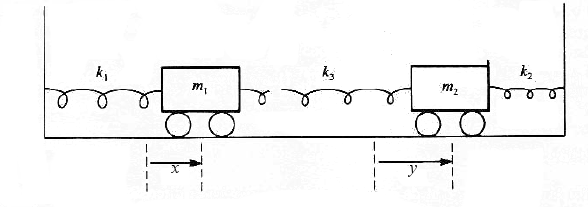
\includegraphics[scale=.5]{/home/fernando/fer/Docencia/grado/EcuacionesDiferenciales/Materiales/Teoria_Basica/imagenes/osci_aco.png}



\begin{equation}
\begin{split} 
             m_1x''(t)&=-k_1x +k_3(y-x) \\
             m_2y''(t)&=-k_3(y-x)-k_2y 
\end{split}\tag{SL}
\end{equation}
 
 
Convertimos en un sistema de primer orden.

$$x_1=x, x_2=x', x_3=y \text{ y } x_4=y'.$$

\begin{equation} 
\left\{
\begin{split} 
            x_1'&=x_2\\
            x_2'&=-\frac{k_1}{m_1}x_1 +\frac{k_3}{m_1}(x_3-x_1) \\
            x_3'&=x_4\\
            x_4'&=-\frac{k_3}{m_2}(x_3-x_1)-\frac{k_2}{m_2}x_3 
\end{split} 
\right.
\end{equation}

\subsection{Modelos Compartimentados}
 
 
 \begin{enumerate}
  \item Se representan gráficamente como un conjunto de cajas \emph{compartimentos} conectados por flechas. 
  \item Puede haber flechas que nacen o  apuntan a un espacio vacío.
 \item Una sustancia viaja por las cajas siguiendo estas flechas. Si la flecha termina en un espacio vacío indica que la sustancia abandona el conjunto de compartimentos. Si la flecha viene del vacío quiere decir que la sustancia ingresa del exterior.
 \item  En cada momento $t$ la sustacia  en cierta caja abandona esta caja siguiendo la dirección de las flechas a una tasa dada.
 \item Si la tasa es proporcional a la cantidad de sustancia que hay en las cajas el \emph{modelo es lineal}.
 \end{enumerate}
 


 \ctikzfig{/home/fernando/fer/Docencia/grado/EcuacionesDiferenciales/Materiales/presentaciones/compartimentos}
 
 \begin{empheq}[left=\empheqlbrace,]{align*}
 x_1'(t)&=-(k_{12}+k_{13})x_1(t)+k_{31}x_3(t)\\
 x_2'(t)&=-k_{23}x_2(t)+k_{12}x_1(t)+q(t)\\
 x'_3(t)&= (k_{13}+k_{23})x_1(t)-(k_{31}+k_{30})x_3(t)
 \label{eq:sist_comp}
   \end{empheq}

\subsection{Un estudio de caso: plomo en sangre}
   
\begin{enumerate}
     \item El plomo es una sustancia tóxica.
     \item Ingresa al torrente sanguíneo desde el aire, agua y  comida.
     \item Se deposita en tejidos, especialmente huesos.
     \item Parte del plomo es eliminado por los riñones.
     \item Otra parte es eliminado con las uñas, pelo y el sudor.
\end{enumerate}




 \begin{empheq}[left=\empheqlbrace,]{align*}
 x_1'(t)&=-(k_{01}+k_{21}+k_{31})x_1(t)+k_{13}x_3(t)+k_{12}x_2(t)+I\\
 x_2'(t)&=-(k_{12}+k_{02})x_2(t)+k_{21}x_1(t)\\
 x'_3(t)&= -k_{13}x_3(t)+k_{31}x_1(t)
   \end{empheq}

\ctikzfig{/home/fernando/fer/Docencia/grado/EcuacionesDiferenciales/Materiales/presentaciones/plomo}

 
\vspace{-20cm}
 


 
 Michael Rabinowitz, George Wetherill, and Joel Kopple.  Estudio controlado de absorción y secreción de plomo del sur de California. Estimaron  $I$ en microgramos/día y las tasas  $k_{j i}$ in 1/día. Los resultados:
 
$$
\begin{aligned}
I_1 &=49.3 ; \quad k_{01}=0.0211, \quad k_{21}=0.0111, \quad k_{31}=0.0039 \\
k_{02} &=0.0162, \quad k_{12}=0.0124, \quad k_{13}=0.000035
\end{aligned}
$$

Resolvemos numéricamente el modelo en un periodo de 800 días con dos condiciones iniciales diferentes
\[
 x(0)=(0,0,0),\quad x(0)=(1800,800,1000).
\]
 

\begin{sympyblock}[][numbers=left,frame=single,framesep=5mm]
from scipy.integrate import odeint 
import numpy as np
import matplotlib.pyplot as plt
\end{sympyblock}


\begin{sympyblock}[][numbers=left,frame=single,framesep=5mm]
def ecuacion(x,t,k,I):
    x1,x2,x3=x
    k01,k21,k31,k02,k12,k13=k
    x1prima=-(k01+k21+k31)*x1+k13*x3+k12*x2+I
    x2prima=-(k12+k02)*x2+k21*x1
    x3prima= -k13*x3+k31*x1
    return x1prima, x2prima, x3prima 
\end{sympyblock}

 

\begin{sympyblock}[][numbers=left,frame=single,framesep=5mm]
I=49.3
k=0.0211,0.0111,0.0039,.0162,0.0124,0.000035 
t=np.linspace(0,800,101)
x0=[0,0,0]
x=odeint(ecuacion,x0,t,args=(k,I))
fig, ax = plt.subplots(1,1)
ax.plot(t,x[:,0],marker='o')
ax.plot(t,x[:,1],marker='^')
ax.plot(t,x[:,2],marker='s')
\end{sympyblock}
 
\begin{sympyblock}[][numbers=left,frame=single,framesep=5mm]
x0=[1800,800,1000]
x=odeint(ecuacion,x0,t,args=(k,I))
ax.plot(t,x[:,0],marker='>')
ax.plot(t,x[:,1],marker='<')
ax.plot(t,x[:,2],marker='+')
ax.legend(('Sangre1','Tejidos1','Huesos1',\
    'Sangre2','Tejidos2','Huesos2'))
plt.savefig('plomo2.pdf', bbox_inches='tight')
\end{sympyblock}

\begin{center}
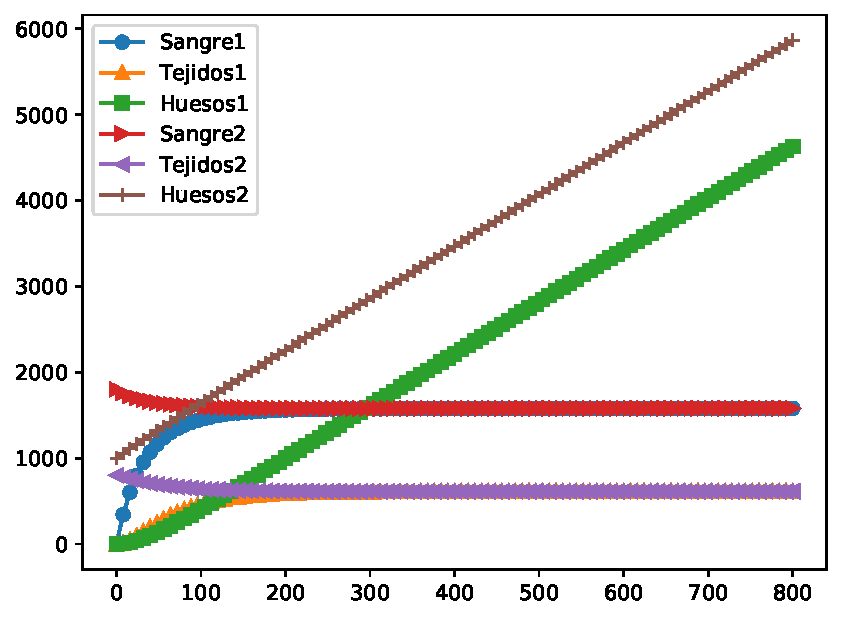
\includegraphics[scale=.5]{plomo2.pdf}
\end{center}
 

 La conclusión del análisis es que sin importar la condición inicial el plomo en sangre se estaliliza en un valor de 1800$\mu$g y en tejidos 800$\mu$g. El plomo en huesos parece crecer a infinito.






\section{Sistemas y ecuaciones de orden $n$}

En general una ecuación lineal de orden $n$

$$
x^{(n)}(t)=a_{n-1}(t) x^{(n-1)}(t)+a_{n-2}(t) x^{(n-2)}(t)+\cdots+a_{0}(t) x(t)+b(t).
$$

se transforma en un sistema mediante

$$x_{1}=x, x_{2}=x', \ldots, x_{n}=x^{(n-1)}$$


$$
\left\{
\begin{split}
\dot{x}_{1}&=x_{2} \\
\dot{x}_{2}&=x_{3} \\
\vdots &  \quad\vdots\\
\dot{x}_{n-1}&=x_{n} \\
\dot{x}_{n}&=a_{0}(t) x_{1}+a_{1}(t) x_{2}+\cdots+a_{n-1}(t) x_{n}+b(t)\\
\end{split}
\right.
$$

$$
A(t)=\begin{pmatrix}
0 & 1 & \cdots &\cdots& 0 \\
0 & 0 & 1 & \cdots & 0 \\
a_{0}(t) & a_{1}(t)&a_{2}(t) & \cdots & a_{n-1}(t)
\end{pmatrix}
\quad 
b(t)=\begin{pmatrix} 0\\
\vdots \\
b(t)
\end{pmatrix}
$$


\begin{ejercicio}{} Cuando $b(t)=0$ el problema se llama \emph{ homogéneo}. Demostrar que en este caso  el conjunto
de soluciones es un espacio vectorial 
\end{ejercicio}



 \section{La matriz fundamental}

 \begin{teorema}[Existencia y unicidad para Sistemas Lineales]{} Sea $A:I \rightarrow \mathbb{R}^{n \times n}$, $b: I \rightarrow \mathbb{R}^{n}$ continuas. Entonces para cada $x_{0} \in \mathbb{R}^{n}$ existe una única solucion $x: I \rightarrow \mathbb{R}^{n}$ del PVI.
$$
\left\{
\begin{array}{ll}
 x^{\prime}(t)&=A(t) x(t)+b(t), \\
 x\left(t_{0}\right)&=x_{0}
\end{array}
\right.
$$
\end{teorema}
 
 
\begin{definicion}[Matriz fundamental] Sean $e^0, \ldots e^{n}$ los vectores canónicos de $\mathbb{R}^{n}$, $t_0\in I\subset\mathbb{R}$. Definimos $\Phi^{0}, \ldots, \Phi^{n}:I \rightarrow \mathbb{R}^{n}$ como
las soluciones de los PVI
\[
\left\{
\begin{split}
{x}'(t)&=A(t)x(t) \\
x(t_{0})&=e^{k}
\end{split}
\right.
\]
La \emph{matriz fundamental} se define como
$$
G=\left[\Phi^{1}|\ldots| \Phi^{n}\right]
$$
\end{definicion}

\begin{observa} La matriz fundamental satisface
$$
\left\{
\begin{split}
{G}'(t)&=A(t) G(t) \\
G(t_0)&=I_{n\times n}
\end{split}\right.
$$
\end{observa}

 \begin{ejemplo}{Osciladar armónico}
$$
{x}''+\omega^{2} x=0.
$$
Si $x_{1}=x, x_{2}=\dot{x}$

\begin{equation}\label{eq:osc_arm_eq}
\left\{
\begin{split}
\dot{x}_{1}&=x_{2},\\
\dot{x}_2&=-\omega^{2} x_1\\
\end{split}
\right.
\end{equation}

Sabemos que

\begin{align*}
 x_1(t)&=x_1^0\cos \omega t+x_2^0\sen\omega t,\\
 x_2(t)&=- x_1^0\omega\sen \omega t+x_2^0\omega\cos\omega t,
 \end{align*}
 
Luego

\begin{multline*}
\left(\begin{array}{l}
x_{1} \\
x_{2}
\end{array}\right)=
\left(\begin{array}{ll}
1 & 0 \\
0 & \omega
\end{array}\right)
\left(\begin{array}{cc}
\cos \omega t & \sen \omega t \\
-\sen \omega t & \cos \omega t
\end{array}\right) \left(\begin{array}{l}
x_{1}^{0} \\
x_{2}^{0}
\end{array}\right)\\
=\left(\begin{array}{ll}
1 & 0 \\
0 & \omega
\end{array}\right)   R(-\omega t)\left(\begin{array}{l}
x_{1}^{0} \\
x_{0}^{0}
\end{array}\right)
\end{multline*}

Para encontrar la matriz fundamental hay que resolver las condiciones iniciales \(x(0)=e^{1}\)  y \(x(0)=e^{2}\). La condición $x(0)=e^1 \Rightarrow x_{1}^{0}=1$ y $x_{2}^{0}=0$ y la condición
$x(0)=e^{2} \Rightarrow x_1^0=0$ y $x_0^{2}=1 / \omega$. Luego las columnas de la MF son

\[\Phi_{1}=\left(\begin{array}{ll}1 & 0 \\ 0 & \omega\end{array}\right) R(-\omega t)\left(\begin{array}{l}1 \\ 0\end{array}\right),\quad
\Phi_{2}=\left(\begin{array}{cc}1 & 0 \\ 0 & \omega\end{array}\right) R(-\omega t)\left(\begin{array}{l}0 \\ 1 / \omega\end{array}\right)
\]

Entonces 

\begin{equation}\label{eq:MF_osc_arm_}G=\left[\Phi_{1} \mid \Phi_{2}\right]=\left(\begin{array}{ll}1 & 0 \\ 0 & \omega\end{array}\right) R(-\omega t)\left(\begin{array}{ll}1 & 0 \\ 0 & 1/\omega\end{array}\right)=H R(-\omega t) H^{-1}
\end{equation}

\end{ejemplo}

\begin{teorema}{teo:sol_gen_SL} si $G(t)$ es una matriz fundamental  entonces $\Phi(t)=G(t)x_0$, con $x_{0} \in \mathbb{R}^{n}$, es una solución general del problema homogéneo. 
\[x'=A x.\]
\end{teorema}

\begin{ejercicio}{} Demostrar el Teorema \ref{teo:sol_gen_SL}.
\end{ejercicio}

\begin{corolario}{}
 E1 conjunto de solucions de $x'=A x$  es un subespacio $n$-dimensional.
\end{corolario}

La matriz fundamental es invertible. Para probar esto necesitamos


\begin{lema}{Derivación de determinantes}
 Supongamos la función matricial $A:I\subset\rr^{n\times n}$ descompuesta en bloques columna 
\[A=\left[A_{*1}|\ldots| A_{* n}\right].\]
Supongamos además que $A \in C^{1}\left(I, \mathbb{R}^{n \times n}\right)$. Entonces
\[\frac{d}{dt}\det( A(t))=\sum_{i=1}^n\det(\left[A_{*1}|\ldots|A'_{*i}|\ldots| A_{* n}\right])\]
\end{lema}

\begin{demo} Usaremos la fórmula de Leibniz del determinante
\[
\det(A)=\sum_{\sigma \in S_n}(-1)^{\epsilon(\sigma)} a_{\sigma(1),1} \cdots a_{\sigma(n),n},
\]
donde $S_n$ es el grupo simétrico de orden $n$, esto es el grupo de permutaciones de $n$-elementos y $\epsilon(\sigma)$ es la paridad de la permutación $\sigma$. 


\[
\begin{split}
 \frac{d}{dt} \det(A)&=\sum_{\sigma \in S_{n}}(-1)^{\varepsilon(\sigma)} a'_{\sigma(1),1} a_{\sigma(2),2} \cdots a_{\sigma(n),n}\\
 &=\sum_{\sigma \in S_{n}}(-1)^{\varepsilon(\sigma)} a_{\sigma(1),1} a'_{\sigma(2),2} \cdots a_{\sigma(n),n}\\
   &\quad \vdots \\
 &=\sum_{\sigma \in S_{n}}(-1)^{\varepsilon(\sigma)} a_{\sigma(1),1} a_{\sigma(2),2} \cdots a'_{\sigma(n),n}\\
 &=\sum_{i=1}^n\det(\left[A_{*1}|\ldots|A'_{*i}|\ldots| A_{* n}\right])
\end{split}
\]
\end{demo}

\begin{observa} También vale que
\begin{equation}\label{eq:form_det2}
\frac{d}{dt}\det( A(t))=\sum_{i=1}^n\det
    \begin{pmatrix} A_{1*}\\ 
                    \vdots \\
                    A'_{i*} \\
                    \vdots\\
                    A_{n*}
    \end{pmatrix}
\end{equation}
 
\end{observa}


\begin{teorema}{Fórmula de Liouville} Si $G$ es la matriz fundamental para $x'=Ax$ entonces

\boxedeq{
\det(G(t))=e^{\int_{t_{0}}^{t} \operatorname{tr} A(s) ds}
}{eq:for_liou}

 
\end{teorema}

\begin{demo} Usamos \eqref{eq:form_det2} y que:
$$
G'_{i *}=\sum_{j=1}^{n} a_{i j} G_{j *}
$$
\begin{multline*}
 \frac{d}{dt}\det \left(G(t)\right)= 
 \sum_{i=1}^n\det 
    \begin{pmatrix}
            G_{1*}\\
            \vdots\\
            G'_{i*}\\
            \vdots\\
            G_{n*}\\
   \end{pmatrix}
 = 
  \sum_{i=1}^n\det 
    \begin{pmatrix}
            G_{1*}\\
            \vdots\\
            \sum_{j=1}^na_{ij}G_{j*}\\
            \vdots\\
            G_{n*}\\
   \end{pmatrix}\\
    =\sum_{i=1}^n\sum_{j=1}^na_{ij}\det 
    \begin{pmatrix}
            G_{1*}\\
            \vdots\\
            G_{j*}\\
            \vdots\\
            G_{n*}\\
   \end{pmatrix}
      =\sum_{i=1}^n a_{ii}\det 
    \begin{pmatrix}
            G_{1*}\\
            \vdots\\
            G_{i*}\\
            \vdots\\
            G_{n*}\\
   \end{pmatrix}=\operatorname{tr}(A)
 \end{multline*}

 Integrando sigue el resultado
\end{demo}

\begin{corolario}{}
  $G(t)$ es no singular.
\end{corolario}


\begin{ejemplo}{} Para el oscilador armónico. 

\begin{equation}\label{eq:MF_oscilador}G(t)=\begin{pmatrix}
\cos \omega t & \frac{\sin \omega t}{\omega} \\ 
-\omega \sin \omega t & \cos \omega t\end{pmatrix}.
\end{equation}

$\operatorname{det}(G(t))=\cos ^{2} \omega t+\sec ^{2} \omega t=1$

$$
A=\left(\begin{array}{cc}
0 & 1 \\
-\omega^{2} & 0
\end{array}\right) \Rightarrow \operatorname{tr}(A)=0 \Rightarrow e^{\int_{t_0}^t\operatorname{tr}(A) dt}=1
$$
\end{ejemplo}
 
\section{Problema no homogéneo} 


\begin{teorema}{}  Supongamos $t_0\in I\subset\rr$, $x_0\in\rr^n$, $A: I \rightarrow \mathbb{R}^{n\times n}$ y $b: I \rightarrow \mathbb{R}^{n}$ y que $G(t)$ matriz fundamental de $A(t)$ ($G'=AG$, $G(t_0)=I_{n\times n}$), entonces

\boxedeq{\varphi(t)=G(t)\left[x_{0}+\int_{t_{0}}^{t}(G(s))^{-1} b(s) d s\right]}{eq:sol_nohom}
es solución de
\begin{equation}
\left\{
 \begin{split}
x'(t)&=A(t) x(t)+b(t)\\
x(t_0)&=x_{0}\\
\end{split}
\right.
\end{equation}


\end{teorema}

\begin{demo}
$$
\begin{aligned}
\dot{\varphi}(t) &=\dot{G}(t)\left[x_{0}+\int_{t_{0}}^{t}(G(s))^{-1} b(s) d{s}\right] +G (t)(G(t))^{-1} b(t) . \\
=& A G\left[x_{0}+\int_{t o}^{t}(G(s))^{-1} b(s) d s\right]+b(t) \\
=&A \varphi( t)+b(t)
\end{aligned}
$$

\end{demo}

Escribamos la fórmula \eqref{eq:sol_nohom} 

\[
\varphi(t) =G(t) x_{0}+G(t) \int_{t_{0}}^{t}(G(s))^{-1} b(s) d s \\
=\varphi_{h}(t)+\varphi_{p}(t)
\]

Notar que $\varphi_h$ resuelve el problema homogéneo y $\varphi_p$ el no-homogéneo.


\begin{ejemplo}[Resorte Forzado]{} Se trata de la ecuación
\[
 x''(t)=-\omega^2x(t)+F(t).
\]

Llamando $x_1=x$ y $x_2=x'$, 


\[
 \left\{
\begin{split}
\dot{x}_{1}&=x_{2} \\
\dot{x}_{2}&=-{\omega}^2x_{1}(t)+F(t) \\
\end{split}
\right.
\]
Alternativamente
\[
\frac{d}{dt}
    \begin{pmatrix}
    x_{1} \\
    x_{2}
    \end{pmatrix} =
    \begin{pmatrix}
    0 & 1 \\
    -\omega^{2} & 0
    \end{pmatrix}
    \begin{pmatrix}
    x_{1} \\
    x_{2}\\
    \end{pmatrix}+
    \begin{pmatrix}
    0 \\
    F(t)\\
    \end{pmatrix}
\]

 \[G(t)=H R(-\omega t) H^{-1},\quad
 R(-\omega t)=
 \begin{pmatrix}
\cos \omega t & \sen \omega t \\
-\sen \omega t & \cos \omega t
\end{pmatrix},\quad
H=
 \begin{pmatrix}
1 & 0 \\
0 & \omega
\end{pmatrix}
\]

Hallemos $\varphi_{p}$ cuando $t_{0}=0$.
\[
\varphi_{p}(t)=G(t) \int_{0}^{t}(G(s))^{-1}
                \begin{pmatrix}
                    0 \\
                    F(s)\\
                \end{pmatrix}
              d s
            =\int_{0}^{t} G(t)(G(s))^{-1}                \begin{pmatrix}
                    0 \\
                    F(s)\\
                \end{pmatrix} d s 
\]

Tenemos
\[
G(t)(G(s))^{-1}=H R(-\omega t) H^{-1} H R(\omega s) H^{-1} 
=H R(\omega(s-t)) H^{-1}.
\]

Ahora


\begin{multline*}
\varphi_{p}(t)=H \int_{0}^{t} R(\omega(s-t)) H^{-1}
                \begin{pmatrix}
                    0 \\
                    F(s)\\
                \end{pmatrix} ds
    =H \int_{0}^{t} R(\omega(s-t))
    \begin{pmatrix}
        0 \\
        \frac{F(s)}{\omega}\\
    \end{pmatrix}d s\\
    =\omega^{-1}H \int_{0}^{t}
    \begin{pmatrix}
        -\sen(\omega(s-t))  \\
        \cos (\omega(s-t))  
    \end{pmatrix}F(s)
    ds
    =\omega^{-1} \int_{0}^{t}
    \begin{pmatrix}
        -\sen(\omega(s-t))  \\
        \cos (\omega(s-t))  \\
    \end{pmatrix}F(s)ds
\end{multline*}

Luego

\[
\begin{split}
x_{1}(t)&=-\frac{1}{\omega} \int_{0}^{t} \sen(\omega(s-t)) F(s) d s \\
x_{2}(t)&=\frac{1}{\omega} \int_{0}^{t} \cos (\omega(s-t)) F(s) d s\\
\end{split}
\]
\end{ejemplo}


\section{Sistemas lineales homogéneos con coeficientes constantes}

Son sistenas de la forma
\boxedeq{
x'=Ax, \quad A \in \mathbb{R}^{n \times n}
}{eq:sist_lin_main}

La forma de resolver es considerar la sustitución
\boxedeq{
y=P^{-1} x
}{eq:cambio_var}

donde $P$ es no singular.  Entonces

$$
y'=P^{-1} x'=P^{-1} A x=P^{-1}A Py
$$

Es una ecuación de la forma 
\[y'=By,\quad \text{con } B \sim A.\]

¿Que sistemas sabríamos resolver? Si $B$ fuese diagonal 
\[B=\operatorname{diag} \left\{ \lambda_{1},\ldots \lambda_{n}\right\}\]
Entonces quedaría un sistema \emph{desacomplado} que podríamos resolver

\[
\begin{split}
y'_{1}&=\lambda_{1} y_{1} \\
&\quad \vdots\\
y'_{n}&=\lambda_{n} y_{n} \\
\end{split}
\]
Las soluciones son:
\[y_{j}(t)=A_{j} e^{\lambda_{j} t},\quad A_j\in\rr
\]
 
La matriz fundamental es
\begin{equation}\label{eq:MF_diagona}
G(t)=\begin{pmatrix}
e^{\lambda_{1} t} & \\
& \ddots \\
& e^{\lambda_{n} t}\\
\end{pmatrix}
\end{equation}

Pero desafortunadamente no toda matriz es diogonalizable. 

\begin{ejercicio}{} Demostrar que si $v\in\rr^n$ es un autovector asociado al autovalor $\lambda$ de $A$ entonces $x(t)=e^{\lambda t}v$ es solución de $x'=Ax$. 
 \end{ejercicio}

\subsection{Exponencial de matrices}


La solución de 

$$
\left\{
\begin{split}
    x(t)&=\lambda x(t)  \\
    x(0)&=x_0 \\
\end{split}
\right.
$$
con $\lambda,x_0 \in \mathbb{R}$, $x:\mathbb{R}\to\rr$, es $x(t)=e^{\lambda t} a$. Razonando por analogia, la de

\[
 \begin{split}
  x'&=Ax\\
  x(0)&=x_0\in\rr^n\\
 \end{split}
\]
debería ser 
\[x(t)=e^{A t}x_0\]

Para ello deberíamos darle sentido a la exponencial de una matriz. 

Recordemos que sobre el espacio de las matrices cuadradas se dice que una norma se llama \emph{norma matricial} si satisface
\[    
  \|AB\|\leq \|A\|\|B\|.
\]
Hay muchas normas matriciales, todas equivalentes. Por ejemplo
\[
 \|A\|=\sup\{\|Ax\| \mid  x\in\rr^n, \|x\|=1\}.
\]
Estas normas dotan a $\rr^{n\times n}$ de una estructura de \emph{espacio de Banach}, es decir es un espacio normado completo. 



\begin{definicion}{Convergencia de series de matrices} Sean $A_j\in\rr^{n\times n}$, $j=0,1,\ldots$ una sucesión de matrices. Diremos que la serie 
\[
 \sum_{j=0}^{\infty} A_j
\]
converge si la sucesión de sumas parciales
\[
 S_m=\sum_{j=0}^{m} A_j
\]
 converge en el espacio métrico de las matrices dado por una norma matricial. 
\end{definicion}


\begin{teorema}{Exponencial de matrices} Sea $A\in\rr^{n\times n}$. Entonces  la serie matricial
\[
\sum_{n=0}^{\infty} \frac{A^n}{n!}=I+A+\frac{A^{2}}{2 !}+\cdots\]
converge. La matriz resultante se denomina exponencial de $A$ y se denota $e^A$.
\end{teorema}

\begin{demo} Veamos que la sucesión de sumas parcales es de Cauchy. Sean $M>N$. 
$$
\left\|S_{M}-S_{N}\right\|=\left\|\sum_{j=N+1}^{M} \frac{A^{j}}{j!}\right\| \leqslant \sum_{j=N+1}^{M} \frac{\| A \|^j}{j !}
$$
 y la última suma puede hacerse tan  chica como queramos pues la serie
 \[
  e^{\|A\|}=\sum_{n=0}^{\infty}\frac{\|A\|^n}{n!}
 \]
es convergente
\end{demo}


\begin{ejemplo}{Matriz diagonal}  Si
 $$
 A=\begin{pmatrix}
\lambda_{1}&0 & \cdots \\
\vdots & \ddots& \vdots\\
0 &\cdots & \lambda_{n}\\
\end{pmatrix}
$$

Entonces 

 $$
 A^j=\begin{pmatrix}
\lambda^j_{1}&0 & \cdots \\
\vdots & \ddots& \vdots\\
0 &\cdots & \lambda^j_{n}\\
\end{pmatrix}
$$
Luego si $t\in\rr$

 $$
 e^{tA}=\sum_{j=0}^{\infty}\frac{t^j}{j!}\begin{pmatrix}
\lambda^j_{1}&0 & \cdots \\
\vdots & \ddots& \vdots\\
0 &\cdots & \lambda^j_{n}\\
\end{pmatrix}=
\begin{pmatrix}
\sum_{j=0}^{\infty}\frac{t^j}{j!}\lambda^j_{1}&0 & \cdots \\
\vdots & \ddots& \vdots\\
0 &\cdots & \sum_{j=0}^{\infty}\frac{t^j}{j!}\lambda^j_{n}\\
\end{pmatrix}
=
\begin{pmatrix}
e^{\lambda_{1}t}&0 & \cdots \\
\vdots & \ddots& \vdots\\
0 &\cdots & e^{\lambda_n t}\\
\end{pmatrix}
$$
Que resulta ser la matriz fundamental del sistema $x'=Ax$.
\end{ejemplo}


\begin{ejemplo}{Oscilador armónico}
Calculemos aproximaciones de la exponencial con SymPy para el sistema
\[
 \begin{pmatrix}
  x_1(t)\\
  x_2(t)
 \end{pmatrix}'=\begin{pmatrix}
 0 & 1\\
 -\omega^2 & 0\\
  \end{pmatrix}
 \begin{pmatrix}
  x_1(t)\\
  x_2(t)
 \end{pmatrix}
\]

\begin{sympyblock}[][numbers=left,frame=single,framesep=5mm]
from sympy import *
omega,t=symbols('omega,t')
A=Matrix([[0, 1],[-omega**2,0]])
G=t**0*A**0
for j in range(1,10):
    G=G+t**j*A**j/factorial(j)
\end{sympyblock}

Se obtiene
\begin{equation}\label{eq:MF_resort}
 \sum_{j=0}^{10}t^j\frac{A^j}{j!}=\sympy{G}.
\end{equation}
Comparar  con \eqref{eq:MF_oscilador}.
\end{ejemplo}


\begin{ejemplo}{Matrices nilpotentes} Una matriz $N\in\rr^{n\times n}$ se llama \emph{nilpotente de orden $r\in\nn$}
si $ 0 \neq N, O\neq N^{2}, \ldots, O \neq N^{r-1}$ y $ 0=N^{r}$.
Si $N$ es milpotente entonces
$$
e^{t N}=I+t N+\frac{t^{2}}{2} N^{2}+\cdots+\frac{t^{r-1}}{(r-1) !} N^{r}
$$


La matriz
$$
N=\begin{pmatrix}
0 & 1 & \cdots &\cdots & 0 \\
0 & 0 & 1 & \cdots & 0 \\
\vdots &\vdots &\vdots &\ddots &0\\
0 & 0 & \cdots & \cdots &  1 \\
0 & \cdots & \cdots & \cdots &0\\
\end{pmatrix},
$$
es nilpotente. Notar que sobre un vector  opera
$$
N\begin{pmatrix}
x_{1} \\
\vdots\\
\vdots\\
x_{n}
\end{pmatrix}=
\begin{pmatrix}
x_{2} \\
x_{3} \\
\vdots\\
x_n\\
0\\
\end{pmatrix}
$$
Luego
\[
\begin{split}
    N^2&=\begin{pmatrix}
0 & 0&  1 & \cdots &\cdots & 0 \\
0 & 0 & 0 & 1 & \cdots & 0 \\
\vdots &\vdots &\vdots &\vdots &\ddots &0\\
0 & 0 & 0 & \cdots & \cdots &  1 \\
0 & \cdots & \cdots& \cdots & \cdots &0\\
0 & \cdots & \cdots & \cdots & \cdots &0\\
\end{pmatrix},\\
\quad \vdots &\qquad\qquad\qquad  \vdots \\
    N^{n-1}&=\begin{pmatrix}
0 & 0&  0 & \cdots &\cdots & 1 \\
0 & 0 & 0 & 0 & \cdots & 0 \\
\vdots &\vdots &\vdots &\vdots &\ddots &0\\
0 & 0 & 0 & \cdots & \cdots &  0 \\
0 & \cdots & \cdots& \cdots & \cdots &0\\
0 & \cdots & \cdots & \cdots & \cdots &0\\
\end{pmatrix},\\
N^n&=\boldsymbol{0}
\end{split}
\]
Luego

\[
\begin{split}
e^{N t}&=I+t N+\frac{t^{2}}{2!} N^{2}+\cdots+\frac{t^{n-1}}{(n-1)!} N^{n-1}\\
        &=\begin{pmatrix}
        1 & \cdots & 0\\
        0 & \ddots & 0 \\
        0&\cdots  & 1
        \end{pmatrix}+
        \begin{pmatrix}
        0 & t & \cdots & 0 \\
        \vdots & \vdots &\ddots & \vdots \\
        0 & \cdots & \cdots & t \\
        0 & \cdots & \cdots & 0 \\
        \end{pmatrix}+
        \begin{pmatrix}
        0 &\cdots &  \frac{t^{n-1}}{(n-1) !} \\
        0 & \cdots &  0 \\
        0 & \cdots &  0 \\
        0 & \cdots &  0 \\
        \end{pmatrix}.\\
        &=
        \begin{pmatrix}
            1 & t & \frac{t^2}{2!} & \cdots & \frac{t^{n-1}}{(n-1) !}  \\
            \vdots & \vdots &\ddots&\ddots & \vdots \\
              0 & \cdots &  \cdots &\cdots & \frac{t^2}{2!} \\
            0 & \cdots &  \cdots &\cdots & t \\
            0 & \cdots  & \cdots& \cdots & 1 \\
        \end{pmatrix}
\end{split}
\]



\end{ejemplo}


\begin{ejemplo}{ej:aut_compl} Calculemos $e^{R}$ donde
$$
R=\begin{pmatrix}
     \mu & \nu \\ -\nu & \mu\\
    \end{pmatrix}
$$

\begin{definicion}{}
\[
 \mathcal{M}=\left\{
        \begin{pmatrix}
     \mu & \nu \\ -\nu & \mu\\
    \end{pmatrix}
    \mid
    \mu, \nu \in \mathbb{R}
    \right\}.
\]
\end{definicion}

\begin{ejercicio}{} (a) $M$ es  cuerpo. (b) La función:

\begin{eqnarray*}
 f:  \mathbb{C}&\to &\mathcal{M}\\
    \mu+i\nu & \mapsto 
    &\begin{pmatrix}
            \mu & \nu \\ -\nu & \mu\\
    \end{pmatrix}
 \end{eqnarray*}
es continua y un isomorfismo de cuerpos.


 \end{ejercicio}
$$
R=\begin{pmatrix}
\mu & \nu \\
-\nu & \mu
\end{pmatrix}=f(\mu+\nu i)=f(z)
$$


 
 
 \begin{multline}\label{eq:exp_compl}
    e^{R}   =\lim _{n \rightarrow \infty}\left(I+R+\cdots+\frac{R^{n}}{n!}\right)
           =\lim _{n \rightarrow \infty}\left(f(1)+f(z)+\frac{f^{2}(z)}{2!}+\cdots+\frac{f^n(z)}{n!}\right)\\
           =\lim _{n \rightarrow \infty} f\left(1+z+\frac{z^{2}}{2}+\cdots+\frac{z^{n}}{n !}\right)
           =f\left(\lim _{n \rightarrow \infty}\left(1+z+\cdots+\frac{z^{n}}{n!}\right)\right)\\
           =f\left(e^{z}\right)=f\left(e^{\mu}(\cos \nu+i \sen \nu)\right)
     =
        \begin{pmatrix}
            e^{\mu} \cos \nu & e^{\mu } \sen \nu \\
            -e^{\mu} \sen\nu & e^{\mu} \cos \nu
        \end{pmatrix}
         =e^{\mu}
        \begin{pmatrix}
            \cos \nu & \sen \nu \\
            -\sen \nu & \cos \nu
        \end{pmatrix}
 \end{multline}

\end{ejemplo}


\begin{teorema}[Propiedades de la exponencial]{teo:prop_exp}
\begin{enumerate}
\item $e^{\boldsymbol{0}}=I$,
 \item $e^{P^{-1}AP}=P^{-1} e^{A}P$. En particular  $A \sim B \Rightarrow e^{A}\sim e^{B}$,
 \item Si $A$  conmuta con $B$ $(A B=B A)$ entonces
 \[e^{A+B} =e^{A} e^{B} ,\]
 \item $e^A$ es no singular y $\left(e^A\right)^{-1}=e^{-A}$. 
\end{enumerate}

\end{teorema}

\begin{demo}
Demostremos 2. Observar que
\[
 \left(P^{-1}AP\right)^n=P^{-1}APP^{-1}AP\cdots P^{-1}AP=P^{-1}A^nP
\]
Luego
\[e^{P^{-1} A P}= \sum_{n=0}^{\infty}\frac{ \left(P^{-1} A P\right)^n}{n!}
= \sum_{n=0}^{\infty}\frac{P^{-1} A^n P}{n!} 
=P^{-1} \left(\sum_{n=0}^{\infty}\frac{ A^n}{n!}  \right)P=P^{-1}e^AP.
\]


Demostremos 3. Usando la formula del binomio de Newton 
\[(A+B)^{n}=\sum_{j=0}^{n} \binom{n}{j} A^{j} B^{n-j}\]
Luego
$$
e^{A+B}=\sum_{n=0}^{\infty}\frac{1}{n!} \sum_{j=0}^{n}\binom{n}{j}
A^{j} B^{n-j}
$$
Por otro lado
$$
\begin{aligned}
e^{A}  e^{B}&=\left(I+A+\frac{A^{2}}{2 !}+\frac{A^{3}}{3 !}+\cdots\right)\left(I+B+\frac{B^{2}}{2}+\frac{B^{3}}{3}+\cdots\right) \\
&=I+A+B+\frac{A^{2}}{2}+A B+\frac{B^{2}}{2}+\frac{A^{3}}{3 !}+\frac{A^{2}}{2 !} B+A \frac{B^{2}}{2 !}+\frac{B^{3}}{3}+\cdots\\
&=\sum_{n=0}^{\infty} \frac{1}{n!}\sum_{j=0}^{n}\binom{n}{j} A^j B^{n-j}=e^{A+B}
\end{aligned}
$$
 \end{demo}



\begin{teorema}[Exponencial y matriz fundamental]{} Si $A\in\rr^{n\times n}$ entonces
 \[
  \frac{d}{d t} e^{A t}=A e^{A t} =e^{A t} A \\ 
 \]
Luego si $G(t)=e^{A t}$, como $G(0)=I$,  $G(t)$ es la matriz fundamental para
el sistema $x'=Ax$ en $t_0=0$.
\end{teorema}

\begin{demo}
\begin{multline*}
\frac{d}{d t} e^{t A}=\lim _{h \rightarrow 0} \frac{e^{(t+h) A}-e^{t A}}{h}=\lim _{h \rightarrow 0} \frac{e^{h A} e^{t A}-e^{t A}}{h}
=\left[\lim _{n \rightarrow 0}\left(\frac{e^{h A}-I}{h}\right)\right] e^{t A}\\
=\lim _{h \rightarrow 0} \frac{\left(h A+\frac{h^2}{2} A^{2}+\cdots\right)}{h} e^{t A}
=A \lim _{h \rightarrow 0}\left(I+h(A+\cdots)) e^{t A}=A e^{t A}\right.
\end{multline*}
\end{demo}

\section{Exponenciales y formas de Jordan}

Un bloque elemental  de Jordan asociado a un autovalor real $\lambda\in\rr$ es una matriz  de la siguiente forma
\[
\begin{split}
 J&=
   \begin{pmatrix}
    \lambda & 1        & \cdots& \cdots  &0\\
    0         &\lambda  &  1      &\cdots &0 \\
    \vdots    & \vdots   &\ddots  &\ddots&\vdots \\
     \vdots    & \vdots  & \vdots   &\lambda  &1\\
      0    & 0   & \cdots& \cdots &\lambda\\   
   \end{pmatrix}\\
   &=
      \begin{pmatrix}
    \lambda & 0        & \cdots& \cdots  &0\\
    0         &\lambda  &  0      &\cdots &0 \\
    \vdots    & \vdots   &\ddots  &\ddots&\vdots \\
     \vdots    & \vdots  & \vdots   &\lambda  &0\\
      0    & 0   & \cdots& \cdots &\lambda\\   
   \end{pmatrix}
  +
      \begin{pmatrix}
    0 & 1        & \cdots& \cdots  &0\\
    0         &0  &  1      &\cdots &0 \\
    \vdots    & \vdots   &\ddots  &\ddots&\vdots \\
     \vdots    & \vdots  & \vdots   &0  &1\\
      0    & 0   & \cdots& \cdots &0\\   
   \end{pmatrix}\\
   &=\lambda I+N.
\end{split}
\]
Como $t\lambda I$ y $tN$ conmutan
\[e^{tJ}=e^{t(\lambda I+N)}=e^{t\lambda I}e^{tN}.\]
Cada uno de los factores $e^{t\lambda I}$ y $e^{tN}$ los hemos calculado. 

Un bloque elemental  de Jordan asociado a un autovalor complejo $\lambda=\mu+i\nu\in\mathbb{C}$ es una matriz  de la siguiente forma
\[
\begin{split}
 J&=
   \begin{pmatrix}
    R & I        & \cdots& \cdots  &\boldsymbol{0}\\
    \boldsymbol{0}         &R  &  I      &\cdots &\boldsymbol{0} \\
    \vdots    & \vdots   &\ddots  &\ddots&\vdots \\
     \vdots    & \vdots  & \vdots   &R  &I\\
      \boldsymbol{0}    & \boldsymbol{0}   & \cdots& \cdots &R\\   
   \end{pmatrix}\\
   &=
      \begin{pmatrix}
    R & \boldsymbol{0}        & \cdots& \cdots  &\boldsymbol{0}\\
    \boldsymbol{0}         &R  &  \boldsymbol{0}      &\cdots &\boldsymbol{0} \\
    \vdots    & \vdots   &\ddots  &\ddots&\vdots \\
     \vdots    & \vdots  & \vdots   &R  &\boldsymbol{0}\\
      \boldsymbol{0}    & \boldsymbol{0}   & \cdots& \cdots &R\\   
   \end{pmatrix}
  +
      \begin{pmatrix}
    \boldsymbol{0} & I        & \cdots& \cdots  &\boldsymbol{0}\\
    \boldsymbol{0}         &\boldsymbol{0}  &  I      &\cdots &\boldsymbol{0} \\
    \vdots    & \vdots   &\ddots  &\ddots&\vdots \\
     \vdots    & \vdots  & \vdots   &\boldsymbol{0}  &I\\
      \boldsymbol{0}    & \boldsymbol{0}   & \cdots& \cdots &\boldsymbol{0}\\   
   \end{pmatrix}\\
   &=D+N.
\end{split}
\]
En las fórmulas anteriores
\[
 R=\begin{pmatrix}
    \mu & -\nu\\
    \nu & \mu\\
   \end{pmatrix}
,\quad 
  I=\begin{pmatrix}
    1 & 0\\
    0 & 1\\
   \end{pmatrix}
  ,\quad 
   \boldsymbol{0}=\begin{pmatrix}
    0 & 0\\
    0 & 0\\
   \end{pmatrix}
\]
$J$ debe tener una cantidad par de filas y columnas.

\begin{ejercicio}{} Demostrar que si $D,N\in\rr^{2n\times 2n}$
\begin{enumerate}
\item
\[
 \begin{split}
e^{N t}&=I+t N+\frac{t^{2}}{2} N^{2}+\cdots+\frac{t^{n-1}}{n-1} N^{n-1}\\
        &=
        \begin{pmatrix}
            I & tI & \frac{t^2}{2!}I & \cdots & \frac{t^{n-1}}{(n-1) !}I  \\
            \vdots & \vdots &\ddots&\ddots & \vdots \\
              0 & \cdots &  \cdots &\cdots & \frac{t^2}{2!}I \\
            0 & \cdots &  \cdots &\cdots & tI \\
            0 & \cdots  & \cdots& \cdots & I \\
        \end{pmatrix}
\end{split}
\]
\item
\[
 e^{tD}=
\begin{pmatrix}
e^{Rt}&0 & \cdots \\
\vdots & \ddots& \vdots\\
0 &\cdots & e^{R t}\\
\end{pmatrix}
\]
\end{enumerate}
Recordar que $e^{Rt}$ la hemos calculado en el ejemplo \ref{ej:aut_compl}.
 
\end{ejercicio}

El Teorema de Jordan asegura que dada cualquier matriz existe una matriz no singular $P$ tal que $P^{-1}AP=J$, donde $J$ es una matriz diagonal por bloques, 
\[J=\operatorname{diag}\{J_1,J_2,\ldots,J_r\},\]
y cada bloque $J_k$ es un bloque elemental de Jordan asociado a algún autovalor. A un mismo autovalor de $A$ pueden estar asociados varios bloques elementales de Jordan. Para la descripción precisa de la matriz $J$ y para una discusión de como calcularla ver \cite{CarlD.Meyer538}, también ver \cite{alg_lin_repaso}.

\section{Clasificación de los retratos de fases de los sistemas planos}

\subsection{Retratos de fases}

En física el espacio de fases es un sistema cartesianos donde se representan variables posicionales y sus velocidades. En el espacio de fases no se representa el tiempo.  Por ejemplo, en el caso del sistema masa-resorte hay una variable posicional, digamos $x$. Por consiguiente, el espacio de fases del resorte es un espacio euclideano 2-dimensional, una coordenada  para la posición  $x$ y otro para $x'$.  En general llamaremos \emph{espacio de fases} asociado a un sistema bidimensional de ecuaciones $x'=Ax+b(t)$ al espacio euclideano $\rr^2$ donde las coordenadas representadas en los ejes del sistema cartesiano son las dos coordenadas de la variable dependiente  $x=(x_1,x_2)$ del sistema de ecuaciones. Una \emph{trayectoria} u \emph{órbita} del sistema es la representación gráfica del conjunto $\{(x_1(t),x_2(t)\mid t\in\rr\}$, donde $(x_1,x_2)$ es una solución. Un  \emph{retrato de fases} es representar diversas trayectorias en el espacio de fases. El estudio del retrato de fases es muy importante para entender propiedades de las soluciones, especialmente coando el sistema es \emph{autónomo}. Un sistema lineal es autónomo cuando es homogéneo.

\begin{ejemplo}{} Vamos a usar SymPy para hacer un retrato de fases del sistema \eqref{eq:osc_arm_eq} (con $\omega=1$). Usamos \eqref{eq:MF_osc_arm_} para calcular la matriz fundamental.


\begin{sympyverbatim}[][numbers=left,frame=single,framesep=5mm]
from sympy import *
t=symbols('t')
H=Matrix([[1, 0],[0,1]])
R=Matrix([[cos(t), sin(t)],[-sin(t),cos(t)]])
G=H*R*H.inv()
Phi=G*Matrix([[.1],[0]])
P=plot_parametric(Phi[0],Phi[1],(t,0,2*pi),show=False,\
    aspect_ratio=(1,1))
X=[0.1*n for n in range(1,20)]
for x0 in X:
    Phi=G*Matrix([[x0],[0]])
    P.append(plot_parametric(Phi[0],Phi[1],(t,0,2*pi),\
        show=False,aspect_ratio=(1,1))[0])
P.show()
\end{sympyverbatim}
\begin{figure}[h]
\begin{center}
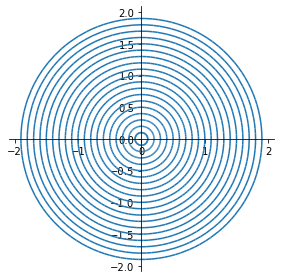
\includegraphics{imagenes/RetratoFasesOsc.png}
\end{center}
\caption{Retrato de fases para el oscilador armónico}\label{fig:osc_arm}
\end{figure}
\end{ejemplo}



\subsection{Polinomio característico de una matriz $A\in A\in\rr^{2\times 2}$}

Dada $A\in\rr^{2\times 2}$ su polinomio característico es
\boxedeq{
P(\lambda)=\det(A-\lambda I)=\lambda^{2}-\operatorname{tr}(A) \lambda+\det(A)=:\lambda^{2}-\tau \lambda+\delta}{eq:pol_car}


Donde la \emph{traza}, \emph{determinante} y \emph{discriminate} son 
\[
\tau=\operatorname{tr}(A), \quad \delta=\det(A),\quad \text { y }\quad \Delta=\tau^{2}-4 \delta. 
\]
Los autovales 

\[
\lambda_1=\frac{\tau - \sqrt{\Delta}}{2}, \quad \lambda_2=\frac{\tau + \sqrt{\Delta}}{2}
\] 
stisfacen
\[
\lambda_1\leq\lambda_2,\quad \lambda_{1}+\lambda_{2}=\tau,\quad  \lambda_{1} \lambda_2=\delta.
\]


\subsection{Caso  $\delta<0$}

En esta situación tendremos que  $\lambda_{1}<0<\lambda_{2}$, y la matriz $A$ es diagonalizable. Luego existe $P\in \operatorname{Gl}(2,\rr)$ tal que 
\[
 \begin{pmatrix}
  \lambda_1 & 0\\
  0  & \lambda_2\\
 \end{pmatrix}
=P^{-1}AP.
\]
Las columnas de $P$ son autovectores de $A$. Si hacemos el cambio de variables \eqref{eq:cambio_var} acorde a \eqref{eq:MF_diagona} y Teorema \ref{teo:sol_gen_SL} 

\begin{equation}\label{eq:sillas1}
y(t)=\begin{pmatrix}
e^{\lambda_1 t} & 0 \\
0 & e^{\lambda_2 t}\\
\end{pmatrix}
\begin{pmatrix}
y_{1}^{0} \\
y_{2}^{0}\\
\end{pmatrix}
=
\begin{pmatrix}
e^{\lambda_1t} y_{1}^{0} \\
e^{\lambda_2 t} y_{2}^{0}\\
\end{pmatrix}
\end{equation}
Es la solución general de  $y'=By=P^{-1}APy$. Observar que $y(0)= (y_{1}^{0},
y_{2}^{0})$.  Eliminando $t$ de las relaciones $y_1(t)= e^{\lambda_1t} y_{1}^{0} $ y $y_2(t)=e^{\lambda_2 t} y_{2}^{0}$ conseguimos (si $y_{1}^{0} \neq 0$)

\begin{equation}\label{eq:sillas2}
 \frac{1}{\lambda_2}\ln\left(\frac{y_2}{y_2^0}\right)=t=\frac{1}{\lambda_1}\ln\left(\frac{y_1}{y_1^0}\right)\Rightarrow  y_2=y_2^0e^{ \frac{\lambda_2}{\lambda_1}  \ln\left(\frac{y_1}{y_1^0}\right) }= y_2^0\left(\frac{y_1}{y_1^0}\right)^\alpha,
\end{equation}
donde $\alpha={\lambda_{2}}/{\lambda_{1}}<0$. Tomamos la parte principal de la función potencia que está bien definida y está en $\rr$ pues siempre $y_1/y_1^0>0$. Tomando en cuenta los signos de $\lambda_1,\lambda_2$
\[
 \lim_{t\to+\infty}y_1(t)=0,\quad \lim_{t\to+\infty}y_2(t)=\lim_{t\to-\infty}y_1(t)=\infty,\quad \lim_{t\to-\infty}y_2(t)=0.
\]

En la figura \ref{fig:silla} representamos un retrato de fases del sistema $y'=By$, cuando $\lambda_1=-2$ y $\lambda_2=1$. Notar que agregamos flechas indicando el recorrido de la curva cuando $t$ va de $-\infty$ a $+\infty$, lo que es una práctica habitual. Si $(y_1^0,y_2^0)=(0,0)$ entonces  $(y_1(t),y_2(t))=(0,0)$ para todo $t$. Esta solución se denomina \emph{estacionaria} pues es constante en el tiempo. También se dice que $(0,0)$ es un \emph{punto de equilibrio}. Esa solución se representada en rojo en el retrato de fases. Observar que dos trayectorias distintas no tienen puntos en común, a menos que sean la misma trayectoria. Esta observación se mantiene cierta para todos sistema de ecuaciones que sea autónomo, esto es que se escriba $x'(t)=f(x(t))$, con $f$ independiente de $t$. En particular ninguna trayectoria   pasa por el $(0,0)$ a menos que sea la trayectoria estacionaria.
Si $y_2^0=0$ entonces $y_2(t)=0$ para todo $t$ y la solución permanece sobre el eje $y_1$. En ese caso se dice que el eje $y_2=0$ es un \emph{subespacio invariante}. De igual manera el eje $y_1=0$ es un subespacio invariante en este caso.


\begin{figure}[h]
\begin{center}
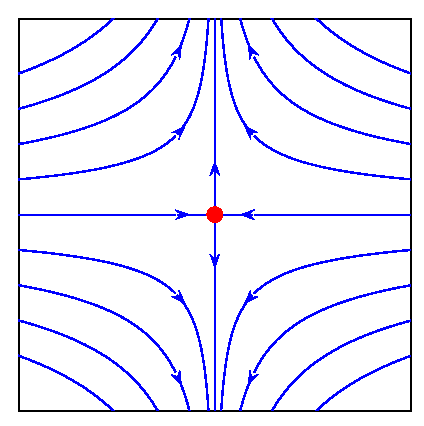
\includegraphics[scale=.7]{imagenes/silla.png}
\caption{Retrato de fases ecuación $y_1'=-2y_1, y_2'=y_2$}\label{fig:silla}
\end{center}
\end{figure}


Recordemos que las variables originales están relacionadas con $y$ por medio de $x=Py$. La transformación $v\mapsto Pv$ lleva los ejes coordenados en las líneas por el $(0,0)$ con la dirección de los autovectores. El retrato de fases correspondiente al sistema original $x'=Ax$ tiene por subespacios invariantes los ejes determinados por los autovectores. Las soluciones se hacen asintóticas cuando $t\to+\infty$ a la línea determinada por el autovector correspondiente al autovalor positivo, es decir $\lambda_2$.  En la figura \ref{fig:silla2} se representa un retrato de fases correspondiente a 
\[
 A=\begin{pmatrix}0 & 1\\2 & -1\end{pmatrix},\quad P=\begin{pmatrix}-1 & 1\\2 & 1\end{pmatrix}.
\]


\begin{figure}[h]
\begin{center}
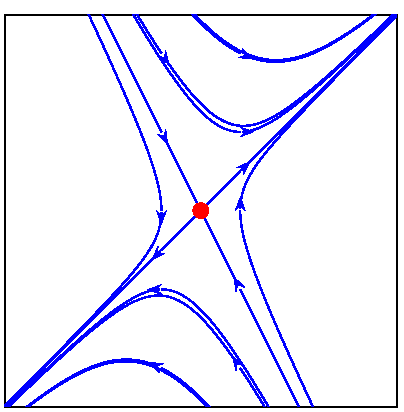
\includegraphics[scale=.7]{imagenes/silla2.png}
\caption{Retrato de fases ecuación $y_1'=y_2, y_2'=2y_1-y_2$}\label{fig:silla2}
\end{center}
\end{figure}

\subsection{Caso $\delta=0$}  La matríz es singular vanuos a  dejar como  ejercicio el estudio de este caso. Observar que el nucleo de la matriz es no trivial y si $(x_1^0,x_2^0)\in\operatorname{Ker}A$ entonces $x(t)\equiv(x_1^0,x_2^0)$ es solución estacionaria. En este caso hay más equilibrios que el $(0,0)$. La figura \ref{fig:lineadeg} representa un retrato de fases de un sistema de estas características.


\begin{figure}[h]
\begin{center}
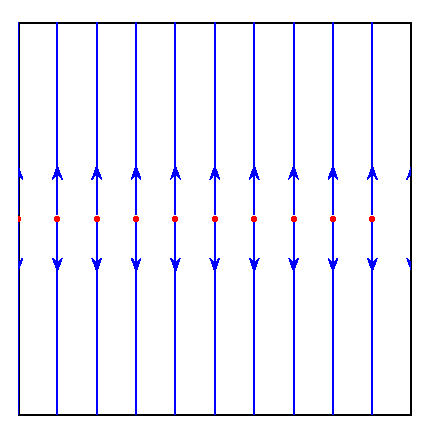
\includegraphics[scale=.7]{imagenes/sist_sing.png}
\end{center}
\caption{Retrato de fases de la ecuación $x_1'=0$,
$x_1'=x_2$}\label{fig:lineadeg}
\end{figure}




\subsection{Caso $\delta>0, \Delta>0$ $(\delta<\frac{\tau^2}{4})$}
Los autovalores son reales, distintos y del mismo signo. El signo de los autovalores es igual al signo de $\tau$. La matriz nuevamente es diagonalizable, la expresión de las soluciones es la misma que en el caso de sillas, es decir para las variables $y$ las expresiones \eqref{eq:sillas1} y \eqref{eq:sillas2},  lo  que cambia es el signo del exponente $\alpha$, ahora $\alpha>0$. Así las  curvas  $y_2= y_2^0\left({y_1}/{y_1^0}\right)^\alpha$  pasan por el origen. Sin embargo, es oportuno remarcar, que una trayectoria corresponde  solo a una rama de esa curva completa, recordar que una trayectoria no puede pasar por $(0,0)$ a menos que sea la solución estacionaria. En este caso tendremos que   
\[
 \lim_{t\to+\infty}y_1(t)=\lim_{t\to+\infty}y_2(t)=\infty\quad\text{y}\quad \lim_{t\to-\infty}y_1(t)=\lim_{t\to-\infty}y_2(t)=0,
\]
cuando $\tau>0$. Cuando $\tau<0$ vale que 
\[
 \lim_{t\to+\infty}y_1(t)=\lim_{t\to+\infty}y_2(t)=0\quad\text{y}\quad\quad \lim_{t\to-\infty}y_1(t)=\lim_{t\to-\infty}y_2(t)=\infty.
\]
La primera situación se dice que el $(0,0)$  es un \emph{nodo inestable} y en la segunda que es un \emph{nodo estable}. En las figuras \ref{fig:nodo_ine} y \ref{fig:nodo_est} se grafican un ejemplo de cada uno. La curvatura de las trayectorias, esto es si son concavas o convexas, depende de si $\alpha>1$ o $\alpha<1$, en la figura \ref{fig:nodo_est_curv2} se grafica un nodo estable con $\alpha<1$.  En la figura \ref{fig:nodo_est_alpha1} se muestra un nodo estable con $\alpha=1$. 


\begin{figure}[h]
 
\begin{subfigure}{.5\textwidth}
\begin{center}
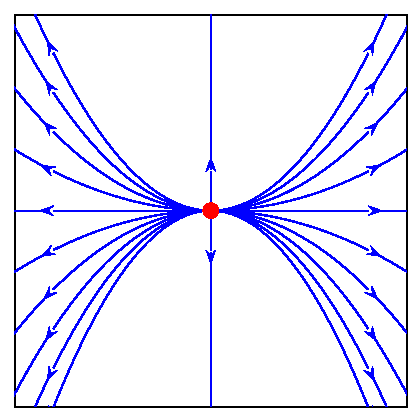
\includegraphics[scale=.5]{imagenes/nodo_ine.png}
\end{center}
\caption{Retrato de fases de la ecuación $x_1'=x_1$,
$x_2'=2x_2$ (nodo inestable)}\label{fig:nodo_ine}
\end{subfigure}
\begin{subfigure}{.5\textwidth}
\begin{center}
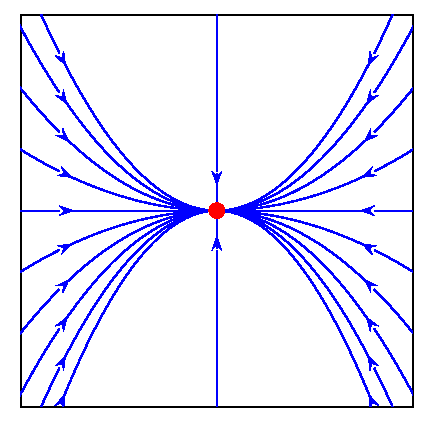
\includegraphics[scale=.5]{imagenes/nodo_est.png}
\end{center}
\caption{Retrato de fases de la ecuación $x_1'=-x_1$,
$x_2'=-2x_2$ (nodo estable)}\label{fig:nodo_est}
\end{subfigure}

\begin{subfigure}{.5\textwidth}
\begin{center}
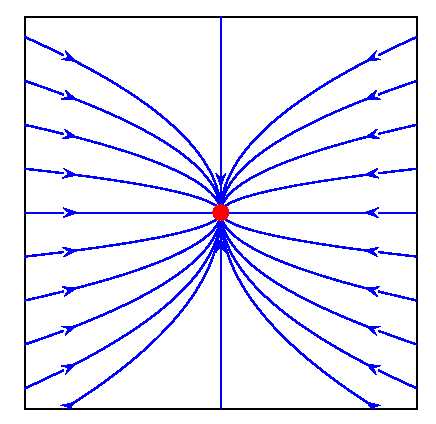
\includegraphics[scale=.5]{imagenes/nodo_est_curv2.png}
\end{center}
\caption{Retrato de fases de la ecuación $x_1'=-2x_1$,
$x_2'=-x_2$ (nodo estable)}\label{fig:nodo_est_curv2}
\end{subfigure}
%
\begin{subfigure}{.5\textwidth}
\begin{center}
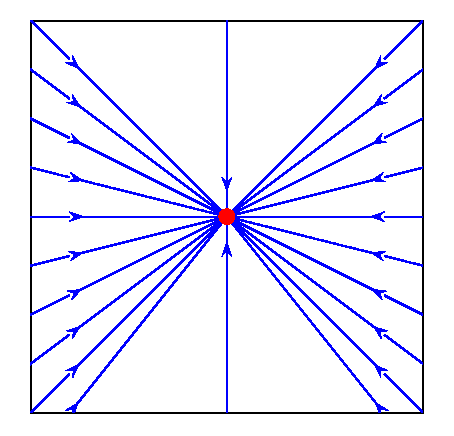
\includegraphics[scale=.5]{imagenes/nodo_est_alpha1.png}
\end{center}
\caption{Retrato de fases de la ecuación $x_1'=-x_1$,
$x_2'=-x_2$ (nodo estable)}\label{fig:nodo_est_alpha1}
\end{subfigure}
\caption{Distintos tipos de nodos}\label{fig:nodos}
\end{figure}


En las figuras \ref{fig:nodos} se representaron retratos de fases cuando $A$ ya estaba en forma diagonal. En esta situación los subespacios invariantes son los ejes de coordenadas. Cuando $A$ no está en su forma diagonal, pero continua en el caso que estamos analizando, los retratos de fases resultan de aplicarle la transformación lineal $P$ a los retratos de  las figuras \ref{fig:nodos}, donde $P$, diagonaliza $A$.   Los subespacios invariantes serán las columnas de $P$ que a la postre son un sistema de autovectores linealmente independiente de $A$. Desarrolllemos un ejemplo con SymPy. En SymPy puden definir matrices y tienen muchas funciones y métodos actiuando sobre estas matrices. Por ejemplo \texttt{A.diagonalize} nos retorna una par de matrices $P$ y $D$ que, por supuesto satisfacen que $D$ es diagonal y $PDP^{-1}=A$, las columnas de $P$ son autovectores de $A$. Por supuesto $A$ podría ser no-diagonalizable, en cuyo caso la función \texttt{diagonalize()} retorna error. 

\begin{ejemplo}{} Consideremos
\[A=
\begin{pmatrix}-2 & -1\\0 & -1\\
 \end{pmatrix}
\]
 

\begin{sympyblock}[][numbers=left,frame=single,framesep=5mm]
A=Matrix([[-2, -1],[0,-1]])
delta=A.det()
tau=A.trace()
delta>0,delta<tau**2/4
\end{sympyblock}
Resulta $(\sympy{delta>0},\sympy{delta<tau**2/4})$. Estamos en el caso $\delta>0$, $\delta<\tau^2/4$. 
\begin{sympyblock}[][numbers=left,frame=single,framesep=5mm]
P,D=A.diagonalize()
\end{sympyblock}

\[
 P=\sympy{P},\quad D=\sympy{D}.
\]

\begin{sympyblock}[][numbers=left,frame=single,framesep=5mm]
tau<0
\end{sympyblock}
Rsulta $\sympy{tau<0}$.  Por todo lo anterior el retrato de fases corresponde a un nodo estable con subespacios invariantes dados por las rectas paralelas a los vectores $(1,0)$ y $(-1,1)$. En la figura \ref{fig:nodo_est_nodiag} representamos el retrato de fases, los subespacios invariantes están indicados en color verde.

\begin{figure}[h]
\begin{center}
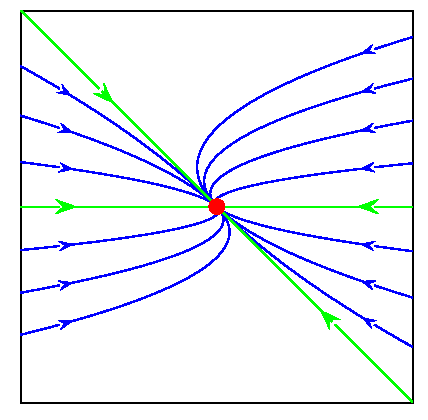
\includegraphics[scale=.5]{imagenes/nodo_est_nodiag.png}
\end{center}
\caption{Retrato de fases de la ecuación $x_1'=-2x_1-x_2$,
$x_2'=-x_2$ (nodo estable)}\label{fig:nodo_est_nodiag}

\end{figure}

\end{ejemplo}



\subsection{Caso $\delta>0, \Delta=0$ $(\delta=\frac{\tau^2}{4})$}

En esta situación los autovalores son iguales $\lambda_1=\lambda_2=:\lambda$. La matriz puede o no ser diagonalizable.Si lo fuera, existiría $P\in \operatorname{Gl}(2,\rr)$ tal que

\[
 \lambda I=
 \begin{pmatrix}
  \lambda & 0\\
  0  & \lambda\\
 \end{pmatrix}
=P^{-1}AP.
\]

Despejando deducimos que $A=\lambda I$. Así nuevamente las soluciones vienen dadas por \eqref{eq:sillas2} con $\lambda=1=\lambda_2$ y el retrato de fases es como el de la figura \ref{fig:nodo_est_alpha1} (podría ser inestable si $\lambda>0$). 

Si $A$ es no diagonalizable, es decir $\lambda$ es un autovalor definiciente o, más concreto aún, la dimensión del autoespacio asociado a $\lambda$ es $1$, entonces el Teorema de Jordan me dice que $A\sim J$ con

\[
 J=\begin{pmatrix} \lambda & 1\\
    0 & \lambda \\
   \end{pmatrix}=
   \begin{pmatrix} \lambda & 0\\
    0 & \lambda \\
   \end{pmatrix}+
   \begin{pmatrix} 0 & 1\\
    0 & 0 \\
   \end{pmatrix}=:D+N
\]
Calculemos $e^{tJ}$. 

\[ e^{tJ}=e^{tD}e^{tN}
 =\begin{pmatrix} e^{\lambda t} & 0\\
    0 & e^{\lambda t} \\
     \end{pmatrix}
      \begin{pmatrix} 1 & t\\
    0 &  1 \\
   \end{pmatrix} = 
   \begin{pmatrix} e^{\lambda t} & te^{\lambda t} \\
    0 & e^{\lambda t} \\
   \end{pmatrix}
\]

La solución general del sistema $y'=Jy$ es:

\[\begin{pmatrix} y_1(t)\\
    y_2(t) \\
   \end{pmatrix}=
 \begin{pmatrix} e^{\lambda t} & te^{\lambda t} \\
    0 & e^{\lambda t} \\
   \end{pmatrix}
\begin{pmatrix} \alpha\\\beta \\
   \end{pmatrix}=
  e^{\lambda t} \begin{pmatrix} \alpha +\beta t \\
                  \beta 
  \end{pmatrix}
  \Rightarrow \left\{ 
  \begin{array}{ll}
   y_1(t)&= e^{\lambda t}\left(\alpha +\beta t\right)\\
   y_2(t)&= \beta e^{\lambda t}\\
  \end{array}
  \right.
\]
Si $y_0^0=0$ entonces $y_2(t)=0$ e $y_1(t)=\alpha e^{\lambda t}$. Luego el eje $y_1$es un subespacio invariante. Si $\beta\neq 0$ entonces $y_2$ no cambia de signo, niunca se cruza el eje $y_1$.  Facilmente se muestra que 
\[
 \lim_{t\to+\infty}y_1(t)=\lim_{t\to+\infty}y_2(t)=\infty\quad\text{y}\quad \lim_{t\to-\infty}y_1(t)=\lim_{t\to-\infty}y_2(t)=0,
\]
si $\lambda>0$ y 
\[
 \lim_{t\to+\infty}y_1(t)=\lim_{t\to+\infty}y_2(t)=0\quad\text{y}\quad \lim_{t\to-\infty}y_1(t)=\lim_{t\to-\infty}y_2(t)=\infty,
\]
si $\lambda<0$


De la segunda ecuación 
\[
 t=\frac{1}{\lambda}\ln\left(\frac{y_2}{\beta}\right).
\]
Reemplazando en la primera, llamando $z=y_2/\beta$, $w=y_1/\alpha$, $\gamma=\frac{1}{\alpha\lambda}$.
\[
 w=\frac{y_1}{\alpha}=y_1=\frac{y_2}{\alpha\beta}\left(\alpha+\frac{\beta}{\lambda}\ln\left(\frac{y_2}{\beta}\right)\right)=z+\gamma z\ln(z)=g(z).
\]
Supongamos $\gamma>0$. Puede verse que $g(z)$ satisface que
\begin{enumerate}
\item 
\[
 g(z)\left\{
            \begin{array}{ll}
             >0, &\text{si } z>e^{-\frac{1}{\gamma}}\\
             =0, &\text{si } z=e^{-\frac{1}{\gamma}}\\ 
             <0, &\text{si } z<e^{-\frac{1}{\gamma}}\\
            \end{array}
\right.
\]
 
 \item $\lim_{z\to 0}g(z)=0$,
 
 \item $g$ es creciente en $(e^{\frac{- \gamma - 1}{\gamma}},+\infty)$ y decreciente en $(-\infty,e^{\frac{- \gamma - 1}{\gamma}},+\infty)$
\end{enumerate}

Todo este análisis explica que el retrato de fases tiene la apariencia de la figura \ref{fig:nodo_est_nodiag2}. Corresponde a un nodo estable, tal como el de la figura  \ref{fig:nodo_est_nodiag} donde los dos subespacios invariantes coinciden.

\begin{figure}[h]
\begin{center}
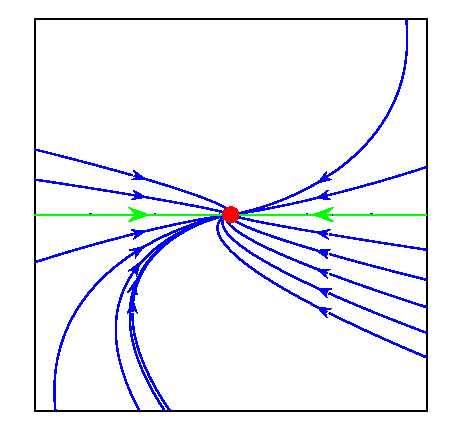
\includegraphics[scale=.5]{imagenes/nodo_est_nodiag2.png}
\end{center}
\caption{Retrato de fases de la ecuación $x_1'=-x_1+x_2$,
$x_2'=-x_2$ (nodo estable)}\label{fig:nodo_est_nodiag2}

\end{figure}



\subsection{Caso $\delta>0, \Delta<0$ $(\delta>\frac{\tau^2}{4})$}

En este caso la matriz es diagonalizable y los autovalores $\lambda=\mu\pm\nu i\in\mathbb{C}\setminus\rr$. Se conoce desde la teoría de diagonalización de matrices (ver \cite{CarlD.Meyer538}) que existe una matriz $P\in \operatorname{Gl}(2,\rr)$ tal que 
\[
 J=\begin{pmatrix}
     \mu & \nu \\ -\nu & \mu\\
    \end{pmatrix}
=
P^{-1}AP
\]
Una manera de obtener $P$ es considerar un autovector $V$ asociado a uno de los autovalores, digamos $\mu+\nu i$, y poner $P=[\operatorname{Re}(V),\operatorname{Im}(V)]$. 

Resulta que el retrato de fases de $x'Ax$ se obtiene  del retrato de fases de $y'=Ry$ aplicádo la transformación $P$. En \eqref{eq:exp_compl} se obtuvo que
\[
       e^{tR}   =e^{\mu t}
        \begin{pmatrix}
            \cos \nu t& \sen \nu t \\
            -\sen \nu t & \cos \nu t
        \end{pmatrix}
\]
 Se tiene que 
 \[
        R(t):=
        \begin{pmatrix}
            \cos \nu & \sen \nu \\
            -\sen \nu & \cos \nu
        \end{pmatrix}
        \in
        \operatorname{O}(2,\rr),
 \]
es decir $R(t)$ es una matriz especial ortogonal ($R^tR=RR^t=I$, $\det(R)=1$),  de hecho $R(t)$ corresponde a una rotación en un ángulo de $\nu t$ alrededor delorigen. Dado un vector fijo de condiciones iniciales $(\alpha,\beta)^t\in\rr^2$ tendremos que la aplicación

\[y: t\mapsto  =e^{\mu t}
        \begin{pmatrix}
            \cos \nu t& \sen \nu t \\
            -\sen \nu t & \cos \nu t
        \end{pmatrix}
        \begin{pmatrix}
            \alpha\\
            \beta
        \end{pmatrix}
    \]
corresponde a una rotación de un ángulo de $\nu t$ seguido de un cambio de escala (homotecia) en un factor de $e^{\mu t}$.  Esto explica que el retrato de fases luzca como xxxxxxx

\begin{ejemplo}{} Consideremos
\[
 A=\begin{pmatrix}1 & 4\\
    -2 & -3
    \end{pmatrix}
\]

\begin{sympyblock}[][numbers=left,frame=single,framesep=5mm]
A=Matrix([[1, 4], [-2, -3]])
delta=A.det()
tau=A.trace()
delta>0,delta>tau**2/4
\end{sympyblock}

Resulta $(\sympy{delta>0},\sympy{delta>tau**2/4})$. Estamos en el caso $\delta>0$, $\delta>\tau^2/4$. 
\begin{sympyblock}[][numbers=left,frame=single,framesep=5mm]
V,D=A.diagonalize()
\end{sympyblock}

\[
 V=\sympy{V},\quad D=\sympy{D}.
\]

Como dijimos arriba hay que considerar

\begin{sympyblock}[][numbers=left,frame=single,framesep=5mm]
P=Matrix([re(V[:,0]).T,im(V[:,0]).T])
\end{sympyblock}
\[
 P=\sympy{P}
\]
\begin{sympyblock}[][numbers=left,frame=single,framesep=5mm]
J=P.inv()*A*P
\end{sympyblock}
\[
 J=\sympy{J}.
\]
Luego la matriz fundamental es
\[
\begin{split}
 G(t)&=\exp(At)=\exp(tPJP^{-1})=P \exp(tJ)P^{-1}\\
 &=e^{-t}\sympy{P}
 \begin{pmatrix}
  \cos(-2t) & \sen(-2t)\\
  -\sen(-2t)  &  \cos(-2t)\\
 \end{pmatrix}
\sympy{P.inv()}\\
&=
e^{-t}\sympy{P*Matrix([[cos(-2*t) , sin(-2*t)],
  [-sin(-2*t),cos(-2*t)]])*P.inv()}
\end{split}
\]

Como cabia imaginar, SymPy sabe calcular exponencial de metrices.

\begin{sympyblock}[][numbers=left,frame=single,framesep=5mm]
t=symbols('t',real=True)
G=exp(t*A)
\end{sympyblock}
Obetenemos
\[
G=\sympy{G},
\]
que coincide con nuestros cálculos previos.



La solución general se obtiene tomando $y_0=(y_0^1,y_0^2)$ y poniendo 
\[
 x(t)=G(t)y_0=e^{-2t}P R(-2t) P^{-1}y_0.
\]
Luego teniendo en cuenta que $R$ es ortogonal
\[
 \|P^{-1}x(t)\|=e^{-2t}\| R(-2t) P^{-1}y_0\|=e^{-2t}\| P^{-1}y_0\|
\]

Entonces $ \|P^{-1}x(t)\|\to 0$ cuando $t\to+\infty$. De  esto se infiere que $ \|x(t)\|\to 0$ cuando $t\to+\infty$.
 
 El retrato de fases es  representado en la figura \ref{fig:foco_est} y se dice que el origen es un \emph{foco estable}.  
\begin{figure}[h]
\begin{center}
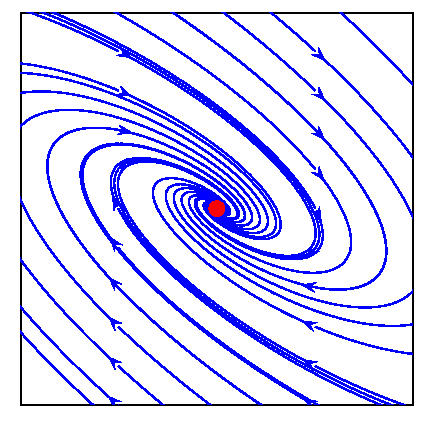
\includegraphics[scale=.5]{imagenes/foco_est.png}
\end{center}
\caption{Retrato de fases de la ecuación $x_1'=x_1+4x_2$,
$x_2'=-2x_1-3x_2$ (foco estable)}\label{fig:foco_est}
\end{figure}

Cuando el autovalor tiene parte real negativa entonces el reatato de fases es similar pero las soluciones tienden a $+\infty$ cuando $t\to +\infty$. Esos casos se llaman \emph{focos inestables}. 

Un caso especial ocurre cuando el autovalor tiene parte real igual a cero. En ese caso la solución general tiene la forma
\[
 x(t)=P
 \begin{pmatrix}
  \cos(\nu t) & \sen(\nu t)\\
  -\sen(\nu t)  &  \cos(\nu t)\\
 \end{pmatrix}
P^{-1}
 \begin{pmatrix}
  \alpha\\
  \beta\\
 \end{pmatrix}
\]

Así en el momento $t$ el vector $w(t):=RP^{-1}(\alpha,\beta)^t$ se determina rotando el vector  $P^{-1}(\alpha,\beta)^t$ un águlo de $\nu t$. Por consiguiente $w(t)$ recorre una circunferencia. La imagen de una circunferencia por la transformación $P$ resulta ser una elipse. Luego la variable $x=Pw$ recorrerá una elipse. En estos casos se dice que el retrato de fases, o el origen, es un \emph{centro}, ver la figura \ref{fig:centro}.


\begin{figure}[h]
\begin{center}
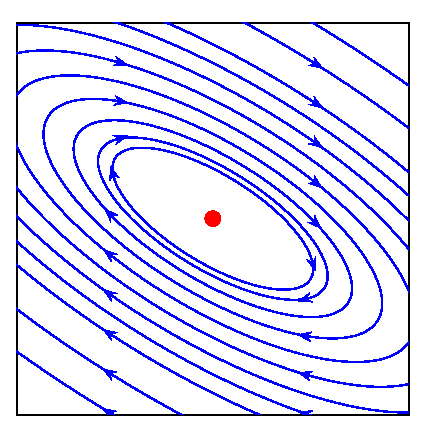
\includegraphics[scale=.5]{imagenes/centro.png}
\end{center}
\caption{Retrato de fases de la ecuación $x_1'=2x_1+4x_2$,
$x_2'=-2x_1-2x_2$ (centro)}\label{fig:centro}
\end{figure}



\end{ejemplo}



\section{El problema no-homogéneo para sistemas con coeficientes constantes}

\begin{corolario}{} Sea $A\in \rr^{n\times n}$ constante, $t_o\in\rr$ y $x_0\in\rr^n$. La solución del PVI
\[
 \left\{
    \begin{array}{ll}
        x^{\prime}&=A x+b(t)\\
        x(t_0)&=x_0\\
    \end{array}
  \right.
\]
viene dada por la expresión
\boxedeq{x(t)=e^{A(t-t_0)} x_0+\int_{t_0}^{t} e^{A(t-s)} b(s) d s}{eq:sol_nohon_const}
\end{corolario}

\begin{demo} Se verifica que la matriz  $G(t)=e^{A(t-t_0)}$ resuelve $G'(t)=AG(t)$ y $G(t_0)=I$. Luego es una matriz fundamental del sistema $x'=Ax$ en $t_0$. Usando la fórmula \eqref{eq:sol_nohom} y  inciso 4. del Teorema \ref{teo:prop_exp} deuducimos
\[
 x(t)=e^{A(t-t_0)}\left[x_0 +\int_{t_0}^t e^{A(t_0-s)}b(s)ds\right]=e^{A(t-t_0)}x_0 +\int_{t_0}^t e^{A(t-s)}b(s)ds
\]

\end{demo}








\section{Ejemplos}

\begin{ejemplo}{ej:retrato_3d} Sea $A\in\rr^{3\times 3}$

\[A=
\begin{pmatrix}- \frac{11}{18} & \frac{34}{45} & - \frac{22}{45}\\- \frac{62}{45} & \frac{53}{90} & - \frac{28}{45}\\- \frac{1}{45} & \frac{23}{45} & - \frac{7}{90}\\
\end{pmatrix}
\]

Usemos la función \texttt{jordan\_form} de SymPy para averiguar la forma de Jordan compleja asociada a $A$.
\begin{sympyblock}[][numbers=left,frame=single,framesep=5mm]
from sympy import *
A=Rational(1,90)*Matrix([[-55, 68, -44],\
    [-124, 53, -56],\
    [-2, 46, -7]])
P1,J1=A.jordan_form()
\end{sympyblock}

\[
 P_1=\sympy{P1},\quad J_1=\sympy{J1}.
\]

El espectro de la matriz $A$ es 

$$\sigma(A)=\sympy{ {J1[i,i] for i in range(3)} }$$

La matriz es diagonalizable. Para llevar a la matriz $A$ a su forma de Jordan real, hay que tomar como $P$ la matriz cuyas columnas son los autovectores asociados a los autovalores reales y para los autovalores complejos tomar la parte real e imaginaria del autovector correspondiente a uno del par de autovalores, digamos en nuestro ejemplo el $-2+i$. Luego

\begin{sympyblock}[][numbers=left,frame=single,framesep=5mm]
P=Matrix([P1[:,0].T,re(P1[:,2]).T,im(P1[:,2]).T]).T
J=P.inv()*A*P
\end{sympyblock}
Obtenemos
\[
 P=\sympy{P},\quad J=\sympy{J}. 
\]
Este resultado nos indica que las soluciones se comportaran como un foco estable en el subespacio generado por los vectores
\[
 V_2=\sympy{P[:,1]}, \quad V_3=\sympy{P[:,2]}.
\]
y como $e^t$ sobre el subespacio generado por 
\[
 V_1=\sympy{P[:,0]}.
\]
 El subespacio $S_1$ generado por $V_1$ y el $S_2$ generado por $\{V_2,V_3\}$ son invariantes. Una solución que inicialmente está en $S_1$ permanece allí y tiende a $+\infty$. En cambio si inicialmente está en $S_2$ permanecerá en el plano $S_2$ describiendo una trayectoria de foco estable.  Es de esperar que una solución cualquiera tienda a $+\infty$ a medida que se va enrollando alrededor del eje generado por $V_1$.

 Observar que
 \begin{sympycode}
t=symbols('t',real=True)
etJ=exp(t*J)
 \end{sympycode}

 
 \[
  e^{tJ}=\sympy{etJ}.
 \]

 Luego

 \begin{multline*}
  e^{tA}=e^{tPJP^{-1}}=Pe^{tJ}P^{-1}\\
  =\sympy{P}\sympy{etJ}\sympy{P.inv()}\\
 \end{multline*}
La matriz que resulta de la multiplicación de matrices del último término es demasiado complicada para dejarla escrito. 

Grafiquemos una solución con condición inicial en $S_2$

\begin{sympyverbatim}
from sympy.plotting import plot3d_parametric_line
G=exp(t*A)
sol=G*P[:,2]
p=plot3d_parametric_line(sol[0],sol[1],sol[2],\
    (t,-10,12),line_color='blue')
sol=G*P[:,0]
p.append(plot3d_parametric_line(sol[0],sol[1],sol[2],\
    (t,-100,12),line_color='red')[0])
sol=G*(P[:,0]+P[:,2])
p.append(plot3d_parametric_line(sol[0],sol[1],sol[2],\
    (t,-10,12),line_color='green')[0])
p.show()
\end{sympyverbatim}



\begin{figure}[h]
\begin{center}
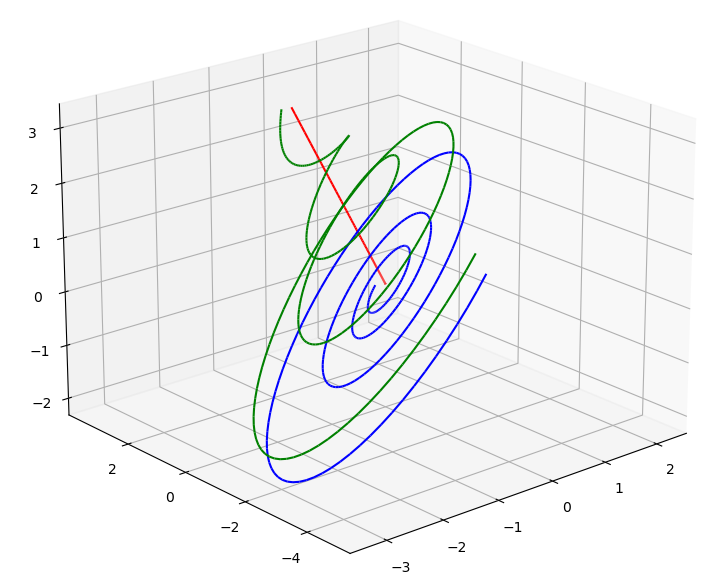
\includegraphics[scale=.5]{imagenes/retrato_3d.png}
\end{center}
\caption{Retrato de fases del ejemplo \ref{ej:retrato_3d}. La linea azul satisface $X(0)=V_3\in S_2$, la roja $x(0)=V_1\in S_1$ y la verde $x(0)=V_1+V_3\in S_1\oplus S_2$, pero $x(0)\notin S_1\cup S_2$}\label{fig:centro}
\end{figure}



 
\end{ejemplo}

\begin{ejemplo}{ej:retrato_3d_aut_def} Sea $A\in\rr^{4\times 4}$ 
 
 \begin{sympycode}
J=Matrix([[-1,1,0,0], [0,-1,0,0],[0,0,1,-2],[0,0,2,1]])
P=Matrix([[-1,1,3,0], [0,-1,0,1],[0,-5,1,-2],[-2,3,2,1]])
A=P.inv()*J*P
 \end{sympycode}

 \[
  A=\sympy{A}.
 \]

 \begin{sympyblock}[][numbers=left,frame=single,framesep=5mm]
from sympy import *
A=Rational(1,13)*Matrix([[11, 115, -56, 61],\
    [-6, 20, 1, 14],\
    [10, 23, -32, 20],\
    [-6, 33, 1, 1]])
P1,J1=A.jordan_form()
\end{sympyblock}
 
 

El espectro de la matriz $A$ es 

$$\sigma(A)=\sympy{ {J1[i,i] for i in range(4)} }$$

El autovalor $-1$ es deficiente, luego la matriz es no diagonalizable. Para llevar a la matriz $A$ a su forma de Jordan real, hay que tomar como $P$ la matriz cuyas columnas son los autovectores asociados a los autovalores reales y para los autovalores complejos tomar la parte real e imaginaria del autovector correspondiente a uno del par de autovalores, digamos en nuestro ejemplo el $1+2i$. Luego

\begin{sympyblock}[][numbers=left,frame=single,framesep=5mm]
P=Matrix([P1[:,0].T,P1[:,1].T,re(P1[:,3]).T,im(P1[:,3]).T]).T
J=P.inv()*A*P
\end{sympyblock} 

Obtenemos
\[
 P=\sympy{P},\quad J=\sympy{J}. 
\]
Este resultado nos indica que las soluciones se comportaran como un foco inestable en el subespacio generado por los vectores
\[
 V_3=\sympy{P[:,2]}, \quad V_4=\sympy{P[:,3]}.
\]
y como un nodo estable del tipo de la figura \ref{fig:nodo_est_nodiag2} sobre el subespacio generado por 
\[
 V_1=\sympy{P[:,0]}\quad{y}\quad V_2=\sympy{P[:,1]}
\]
 El subespacio $S_1$ generado por $\{V_1,V_2\}$ y el $S_2$ generado por $\{V_3,V_4\}$ son invariantes. Una solución que inicialmente está en $S_1$ permanece allí y tiende a $0$ cuando $t\to +\infty$. En cambio si inicialmente está en $S_2$ permanecerá en el plano $S_2$ describiendo una trayectoria de foco inestable.  Es de esperar que una solución cualquiera tienda a $+\infty$ a medida que se va enrollando alrededor de $S_1$\footnote{Habría que precisar que significa enrollarse alrededor de un plano} y cuando $t\to +\infty$, $d(x(t),S_2)\to 0$.

 Observar que
 \begin{sympycode}
t=symbols('t',real=True)
etJ=exp(t*J)
 \end{sympycode}

 
 \[
  e^{tJ}=\sympy{etJ}.
 \]

 Luego
{\small
 \begin{multline*}
  e^{tA}=e^{tPJP^{-1}}=Pe^{tJ}P^{-1}\\
  =\sympy{P}\sympy{etJ}\sympy{P.inv()}\\
 \end{multline*}
 }
La matriz que resulta de la multiplicación de matrices del último término es demasiado complicada para dejarla escrito. 

 
\end{ejemplo}


 
 
\begin{ejemplo}{ej:retrato_3d_aut_def_cplx} Sea $A\in\rr^{4\times 4}$ 
 
 \begin{sympycode}
J=Matrix([[-1,1,1,0], [-1,-1,0,1],[0,0,-1,1],[0,0,-1,-1]])
P=Matrix([[-1,1,3,0], [0,-1,0,1],[0,-5,1,-2],[-2,3,2,1]])
A=P.inv()*J*P
 \end{sympycode}

 \[
  A=\sympy{A}.
 \]

 \begin{sympyblock}[][numbers=left,frame=single,framesep=5mm]
from sympy import *
A=Rational(1,26)*Matrix([[-8, -244, 18, -70],\
[15, -69, 2, -15],\
[1, -119, -12, -27],\
[-11, 9, -24, -15]])
P1,J1=A.jordan_form()
\end{sympyblock}
 
 

El espectro de la matriz $A$ es 

$$\sigma(A)=\sympy{ {J1[i,i] for i in range(4)} }$$

El autovalor $\sympy{J1[0,0]}$ y su conjugados son deficientes, luego la matriz es no diagonalizable. Para llevar a la matriz $A$ a su forma de Jordan real, hay que tomar como $P$ la matriz cuyas columnas son  la parte real e imaginaria de las columnas de $P_1$ correspondientes a uno del par de autovalores, digamos en nuestro ejemplo $\sympy{J1[0,0]}$. Luego

\begin{sympyblock}[][numbers=left,frame=single,framesep=5mm]
P=Matrix([re(P1[:,0]).T,im(P1[:,0]).T,re(P1[:,1]).T,\
    im(P1[:,1]).T]).T
J=P.inv()*A*P
\end{sympyblock} 

Obtenemos
\[
 P=\sympy{P},\quad J=\sympy{J}. 
\]

 Observar que
 \begin{sympycode}
t=symbols('t',real=True)
etJ=exp(t*J)
 \end{sympycode}

 
 \[
  e^{tJ}=\sympy{etJ}.
 \]

 Luego
{\small
 \begin{multline*}
  e^{tA}=e^{tPJP^{-1}}=Pe^{tJ}P^{-1}\\
  =\sympy{P}\times\sympy{etJ}\\ \times \sympy{P.inv()}\\
 \end{multline*}
 }
La matriz que resulta de la multiplicación de matrices del último término es demasiado complicada para dejarla escrito. 

 
\end{ejemplo}





\begin{ejemplo}{} \textbf{Osciladores acoplados}
 
$$
\begin{bmatrix}
\dot{x}_1\\
\dot{x}_2\\
\dot{x}_3\\
\dot{x}_4\\
\end{bmatrix}
=
\begin{bmatrix}
 0 & 1 & 0 & 0\\
 -(\frac{k_1}{m_1}+\frac{k_3}{m_1}) & 0 & \frac{k_3}{m_1} & 0\\
 0&0&0&1\\
  \frac{k_3}{m_2} & 0 &  -(\frac{k_3}{m_2}+\frac{k_2}{m_2}) & 0\\
\end{bmatrix}
\begin{bmatrix}
{x}_1\\
{x}_2\\
{x}_3\\
{x}_4\\
\end{bmatrix}
$$ 
 
Usamos todos los parámetros iguales a 1.
\begin{sympyblock}[][numbers=left,frame=single,framesep=5mm]
k1,k2,k3,m1,m2=symbols('k1,k2,k3,m1,m2',\
    positive=True)
A=Matrix([[0,1,0,0],\
          [-(k1/m1+k3/m1), 0, k3/m1, 0],\
          [0,0,0,1],[k3/m2, 0, -(k3/m2+k2/m2),0] ])
A=A.subs({k1:1,k2:1,k3:1,m1:1,m2:1})
P,D=A.jordan_form()
\end{sympyblock}
 
 $$P=\sympy{P},\quad D=\sympy{D}.$$
 
 Podemos considerar los autovalores $i$ y $\sqrt{3}i$. Tenemos $\mu_1=0$, $\nu_1=1$, $\mu_2=0$, $\nu_2=\sqrt{3}$. Además
$$
Q_1=\begin{pmatrix}
        0\\
        1  \\
        0\\
        1\\
   \end{pmatrix},\quad
R_1=\begin{pmatrix}
        -1\\
        0 \\
        -1\\
        0\\
   \end{pmatrix},\quad
Q_2=\begin{pmatrix}
        0\\
        -1  \\
        0\\
        1\\
   \end{pmatrix},\quad
R_2=\begin{pmatrix}
        \frac{\sqrt{3}}{3}\\
        0 \\
        -\frac{\sqrt{3}}{3}\\
        0\\
   \end{pmatrix},
$$ 
 Obtenemos que la solución general se escribe:

$$
\varphi(t)=c_1\begin{pmatrix}
        \operatorname{sen} t\\
        \cos  t \\
        \operatorname{sen} t\\
        \cos  t\\
   \end{pmatrix}
   +
c_2\begin{pmatrix}
        -\cos  t \\
        \operatorname{sen} t\\
         -\cos  t\\
         \operatorname{sen} t\\
     \end{pmatrix}+
c_3\begin{pmatrix}
        -\operatorname{sen}\frac{\sqrt{3}}{3}t\\
        -\cos \frac{\sqrt{3}}{3} t \\
        \operatorname{sen}\frac{\sqrt{3}}{3} t\\
        \cos \frac{\sqrt{3}}{3} t\\
   \end{pmatrix}
   +
c_4\begin{pmatrix}
        \cos \frac{\sqrt{3}}{3} t \\
        -\operatorname{sen}\frac{\sqrt{3}}{3} t\\
         -\cos \frac{\sqrt{3}}{3} t\\
         \operatorname{sen}\frac{\sqrt{3}}{3} t\\
     \end{pmatrix}
$$
 

Si tomamos $c_3=c_4=0$ la solución  resultará $2\pi$ periódica. 
Observar que en este caso $x=y$ los desplazamientos son iguales.

Si tomamos $c_1=c_2=0$ la solución  resultará $2\pi/\sqrt{3}$ 
periódica. Observar que en este caso $x=-y$ los desplazamientos
son opuestos.

La superposición de dos funciones oscilatorias con frecuencias cuyo 
cociente es un número irracional no resulta periódica (para una 
demostración ver apuntes Ecuaciones Diferenciales 1913). Entonces
$c_3=c_4=0$, $c_1=c_2=0$ son las únicas elecciones que nos dan una 
solución periódica. Se llaman \emph{modos normales de vibración}. 
 
\end{ejemplo}

\begin{ejemplo}{}\textbf{Plomo en sangre}
  
 \begin{quote}
<<Este mal condicionamiento hace que sea muy difícil desarrollar un 
algoritmo numérico robusto para la forma normal de Jordan, 
ya que el resultado depende críticamente de si se considera 
que dos valores propios son iguales. 
Por esta razón, la forma normal de Jordan suele evitarse 
en el análisis numérico....>>
 \end{quote}
 
  \begin{flushright}
   \href{https://en.wikipedia.org/wiki/Jordan_normal_form}{Wikipedia}
  \end{flushright}

\emph{Numpy no implementa Formas de Jordan. 
Con flotantes Sympy tiene dificultades con la función 
\texttt{jordan\_form} }
  
 
 
 
Vamos a resolver el problema de plomo en sangre con $x(0)=(0,0,0)$.

Usaremos la función  \texttt{diagonalize} 
  

\begin{sympyblock}[][numbers=left,frame=single,framesep=5mm]
I=49.3
k01,k21,k31,k02,k12,k13=0.0211,0.0111,0.0039,\
    .0162,0.0124,0.000035 
A=Matrix([[ -(k01+k21+k31), k12, k13],\
    [k21,-(k12+k02), 0],\
    [k31,0,-k13]])
P,D=A.diagonalize()
\end{sympyblock}

\begin{sympycode}
P=P.applyfunc(lambda x: N(x,4))
D=D.applyfunc(lambda x: N(x,4))
\end{sympycode}



 $$\small P=\sympy{P},$$
 
 $$\small D=\sympy{D}.$$
 
 
 
Escribimos la fórmula para el problema no homogéneo.

\begin{sympyblock}[][numbers=left,frame=single,framesep=5mm]
t,s=symbols('t,s',real=True)
G=P*exp(D*t)*P.inv()
Ginv=P*exp(-D*s)*P.inv()
B=Matrix([[I],[0],[0]])
x=G*(Integral(Ginv*B,(s,0,t)).doit()).simplify()
\end{sympyblock}
 



    \begin{eqnarray*}
       x_1(t)=& \tikz[baseline]{
                                \node[fill=yellow, rectangle,anchor=base] (A)
                      {\textcolor{black}%
                      {$8.656 \cdot 10^{-14} e^{0.0247 t}$}}
                      }&\text{(Errores redondeo?)}
                      \\
              &
              \tikz[baseline]{
                                \node[fill=yellow, rectangle,anchor=base] (A)
                      {\textcolor{black}%
                      {$+ 1800.0$}}}& \text{(cantidad límite)} \\
              &- 718.2 e^{- 0.0447 t}&\\ 
              &+ 2.842 \cdot 10^{-14} e^{- 0.0447 t}&\\
              &- 1.362 \cdot 10^{-13} e^{- 0.0247 t}&\\
              &- 856.8 e^{- 0.02 t} &\\
              &+ 4.263 \cdot 10^{-14} e^{- 0.0199 t}& \\
              &- 224.9 e^{- 3.063 \cdot 10^{-5} t}&\\
    \end{eqnarray*}
    

  
 

\emph{Conclusión:} La concentración límite en sangre es de 1800$\mu$g.


 

    \begin{eqnarray*}
       x_2(t)=&\tikz[baseline]{
                                \node[fill=yellow, rectangle,anchor=base] (A)
                      {\textcolor{black}%
                      {$1.137 \cdot 10^{-13} e^{0.0247 t}$}}
                      }&\text{(Errores redondeo?)}
                \\
               & 
               \tikz[baseline]{
                                \node[fill=yellow, rectangle,anchor=base] (A)
                      {\textcolor{black}%
                      {$+ 701.8$}}}& \text{(cantidad límite)} \\               
               & + 496.1 e^{- 0.0447 t}&\\
               &- 1.421 \cdot 10^{-14} e^{- 0.0447 t}&\\
               &+ 1.137 \cdot 10^{-13} e^{- 0.0247 t}&\\
               &- 1111.0 e^{- 0.02 t}&\\
               &+ 7.105 \cdot 10^{-14} e^{- 0.01996 t}&\\
               &- 87.37 e^{- 3.0636 \cdot 10^{-5} t}&
    \end{eqnarray*}
 
\emph{Conclusión:} La concentración límite en tejidos es de 701.8$\mu$g.
  
 


\end{ejemplo}









\begin{ejercicio}{} Sea $A\in \mathbb{R}^{n\times n}$  y supongamos que
$E\subset\mathbb{R}^n$ es un subespacio  invariante por $A$, es decir $v\in E\Rightarrow Av\in E$. Demostrar
que si $x(t)$ es solución de
\[
  \left\{%
\begin{array}{ll}
     x'=Ax \\
    x(0)=C \\
\end{array}%
\right.,
\]
con $C\in E$, entonces $x(t)\in E$ para todo $t$.
\end{ejercicio}


\begin{ejercicio}{} Sea $A\in\mathbb{R}^{n\times n})$. Supongamos que toda solución de
$x'=Ax$ es periódica con el mismo periodo. Demostrar que $A$ es
semisimple y el polinomio característico de $A$ es una potencia
de $t^2+a^2$, $a\in\mathbb{R}$.
\end{ejercicio}


\begin{ejercicio}{} Sea $A\in\mathbb{R}^{n\times n}$. Diremos que la ecuación
\emph{preserva longitudes} si toda solución $x(t)$ satisface que
$|x(t)|=|x(0)|$. Demostrar que las siguientes condiciones son
equivalentes:
\begin{enumerate}
\item La ecuación preserva longitudes.
\item La matriz $e^{tA}$ es ortogonal para todo $t$.
\item $A$ es antisimétrica, es decir $A=-A^t$.
\end{enumerate}
\end{ejercicio}


\begin{ejercicio}{} Supongamos que $\mu$ no es un autovalor de $A$. Demostrar que
\[
    x'=Ax+e^{\mu t}b\quad (b\in\mathbb{R}^n)
\]
tiene una solución de la forma $e^{\mu t}v$, con
$v\in\mathbb{R}^n$.
\end{ejercicio}



\begin{ejercicio} Sea $A\in \mathbb{R}^{4\times 4} $ semisimple y
supongamos que los autovalores de $A$ son $\pm ai$ y $\pm bi$;
$a>0$, $b>0$.  Demostrar que:
\begin{enumerate}
    \item Si $a/b$ es racional entonces toda solución de $x'=Ax$
    es periódica.
    \item Si $a/b$ es irracional, hay una solución no periódica
    $x(t)$ tal que:
        \[
            M<|x(t)|<N
        \]
    para ciertas constantes $M,N>0$.
\end{enumerate}
\end{ejercicio}

 \begin{ejercicio} a) Verificar con SymPy para dos soluciones $x(t)$ distintas a elección del ejemplo \ref{ej:retrato_3d_aut_def} que se verifica que
 \[
  \lim_{t\to+\infty}d(x(t),S_2)=0.
 \]
b) Demostrar la afirmación del inciso a).
 \end{ejercicio}


 
 
 
 
 

